\documentclass[journal]{IEEEtran}
\usepackage{amsmath,amssymb,booktabs,graphicx,xcolor,algorithm,algorithmic,tikz,cite,multirow}
\usetikzlibrary{arrows.meta,positioning}
\newcommand{\nSubjects}{15}
\newcommand{\nWindows}{3101}
\newcommand{\nStressWindows}{926}
\newcommand{\pctStress}{29.9}
\newcommand{\nFeatures}{47}
\newcommand{\nSeeds}{5}
\newcommand{\rawAcc}{89.4}
\newcommand{\rawAccCI}{5.3}
\newcommand{\rawF}{86.6}
\newcommand{\sigmaBVP}{65.2}
\newcommand{\sigmaEDA}{2.34}
\newcommand{\sigmaTEMP}{1.5}
\newcommand{\sigmaACC}{35.7}
\newcommand{\ratioNative}{4.6}
\newcommand{\bpsNative}{6.93}
\newcommand{\accNative}{89.4}
\newcommand{\ratioEa}{8.8}
\newcommand{\bpsEa}{3.63}
\newcommand{\accEa}{89.3}
\newcommand{\dAccEa}{-0.1}
\newcommand{\pAccEa}{0.73}
\newcommand{\fEa}{86.7}
\newcommand{\accMMEa}{88.3}
\newcommand{\savingEa}{88.7}
\newcommand{\maxErrRatioEa}{1.0000}
\newcommand{\ratioEb}{10.5}
\newcommand{\bpsEb}{3.04}
\newcommand{\accEb}{89.2}
\newcommand{\dAccEb}{-0.1}
\newcommand{\pAccEb}{0.78}
\newcommand{\fEb}{86.7}
\newcommand{\accMMEb}{88.7}
\newcommand{\savingEb}{90.5}
\newcommand{\maxErrRatioEb}{1.0000}
\newcommand{\ratioEc}{13.3}
\newcommand{\bpsEc}{2.41}
\newcommand{\accEc}{89.9}
\newcommand{\dAccEc}{0.6}
\newcommand{\pAccEc}{0.20}
\newcommand{\fEc}{87.2}
\newcommand{\accMMEc}{89.8}
\newcommand{\savingEc}{92.5}
\newcommand{\maxErrRatioEc}{1.0000}
\newcommand{\ratioEd}{17.5}
\newcommand{\bpsEd}{1.83}
\newcommand{\accEd}{90.8}
\newcommand{\dAccEd}{1.5}
\newcommand{\pAccEd}{0.07}
\newcommand{\fEd}{88.3}
\newcommand{\accMMEd}{89.9}
\newcommand{\savingEd}{94.3}
\newcommand{\maxErrRatioEd}{1.0000}
\newcommand{\ratioEe}{20.6}
\newcommand{\bpsEe}{1.55}
\newcommand{\accEe}{89.5}
\newcommand{\dAccEe}{0.1}
\newcommand{\pAccEe}{0.44}
\newcommand{\fEe}{86.6}
\newcommand{\accMMEe}{86.7}
\newcommand{\savingEe}{95.2}
\newcommand{\maxErrRatioEe}{1.0000}
\newcommand{\ratioEf}{23.6}
\newcommand{\bpsEf}{1.35}
\newcommand{\accEf}{87.9}
\newcommand{\dAccEf}{-1.4}
\newcommand{\pAccEf}{0.30}
\newcommand{\fEf}{84.8}
\newcommand{\accMMEf}{84.7}
\newcommand{\savingEf}{95.8}
\newcommand{\maxErrRatioEf}{1.0000}
\newcommand{\ratioLossless}{3.23}
\newcommand{\savingLossless}{69.0}
\newcommand{\maxErrRatioAll}{0.999999}
\newcommand{\zfpRatioMin}{3.1}
\newcommand{\zfpRatioMax}{5.3}
\newcommand{\zfpErrMin}{0.46}
\newcommand{\zfpErrMax}{0.57}
\newcommand{\zfpDAccMin}{-0.0}
\newcommand{\zfpDAccMax}{+1.6}
\newcommand{\predGainMin}{1.5}
\newcommand{\predGainMax}{2.0}
\newcommand{\minEDARange}{0.97}
\newcommand{\maxEDARange}{13.1}
\newcommand{\epsEDAEa}{0.01}
\newcommand{\epsBVPEa}{0.33}
\newcommand{\epsTEMPEa}{0.007}
\newcommand{\epsACCEa}{0.18}
\newcommand{\epsEDAEb}{0.02}
\newcommand{\epsBVPEb}{0.65}
\newcommand{\epsTEMPEb}{0.015}
\newcommand{\epsACCEb}{0.36}
\newcommand{\epsEDAEc}{0.05}
\newcommand{\epsBVPEc}{1.30}
\newcommand{\epsTEMPEc}{0.030}
\newcommand{\epsACCEc}{0.71}
\newcommand{\epsEDAEd}{0.12}
\newcommand{\epsBVPEd}{3.26}
\newcommand{\epsTEMPEd}{0.075}
\newcommand{\epsACCEd}{1.79}
\newcommand{\epsEDAEe}{0.23}
\newcommand{\epsBVPEe}{6.52}
\newcommand{\epsTEMPEe}{0.150}
\newcommand{\epsACCEe}{3.57}
\newcommand{\epsEDAEf}{0.47}
\newcommand{\epsBVPEf}{13.03}
\newcommand{\epsTEMPEf}{0.300}
\newcommand{\epsACCEf}{7.15}
\newcommand{\pctSamplesBVPACC}{95.2}
\newcommand{\maxOpenLoopSci}{6.8\times10^{9}}
\newcommand{\minOpenLoopSci}{3.1\times10^{8}}
\newcommand{\nSamplesSci}{1.5\times10^{7}}
\newcommand{\maxOpenLoop}{6836330469}
\newcommand{\minOpenLoop}{313652845}
\newcommand{\dsAccB}{90.0}
\newcommand{\dsPairEpsB}{0.005}
\newcommand{\dsPairRatioB}{8.8}
\newcommand{\dsPairAccB}{89.3}
\newcommand{\dsPairDiffB}{-0.7}
\newcommand{\dsPairPB}{0.13}
\newcommand{\dsAccMMB}{88.7}
\newcommand{\dsPairAbsDiffB}{0.7}
\newcommand{\dsPB}{0.03}
\newcommand{\dsDAccB}{+0.6}
\newcommand{\dsAccC}{92.0}
\newcommand{\dsPairEpsC}{0.005}
\newcommand{\dsPairRatioC}{8.8}
\newcommand{\dsPairAccC}{89.3}
\newcommand{\dsPairDiffC}{-2.7}
\newcommand{\dsPairPC}{0.00}
\newcommand{\dsAccMMC}{86.9}
\newcommand{\dsPairAbsDiffC}{2.7}
\newcommand{\dsPC}{0.01}
\newcommand{\dsDAccC}{+2.6}
\newcommand{\dsAccE}{92.9}
\newcommand{\dsPairEpsE}{0.005}
\newcommand{\dsPairRatioE}{8.8}
\newcommand{\dsPairAccE}{89.3}
\newcommand{\dsPairDiffE}{-3.6}
\newcommand{\dsPairPE}{0.01}
\newcommand{\dsAccMME}{84.8}
\newcommand{\dsPairAbsDiffE}{3.6}
\newcommand{\dsPE}{0.01}
\newcommand{\dsDAccE}{+3.6}

\newcommand{\allocNCombos}{10000}
\newcommand{\allocNLevels}{10}
\newcommand{\allocBestTarget}{28}
\newcommand{\allocBestGain}{+3.7}
\newcommand{\allocBestP}{0.421}
\newcommand{\allocPooledDiff}{+0.6}
\newcommand{\allocPooledP}{0.632}
\newcommand{\allocPooledDiffFeat}{+0.9}
\newcommand{\allocPooledPFeat}{0.448}
\newcommand{\allocUniformAccD}{89.7}
\newcommand{\allocUniformRatioD}{8.8}
\newcommand{\allocFeatAccD}{89.3}
\newcommand{\allocFeatRatioD}{6.4}
\newcommand{\allocClfAccD}{89.3}
\newcommand{\allocClfRatioD}{6.4}
\newcommand{\allocClfSavingD}{84.3}
\newcommand{\allocClfDiffD}{-0.4}
\newcommand{\allocClfPD}{0.07}
\newcommand{\allocUniformAccF}{89.7}
\newcommand{\allocUniformRatioF}{8.8}
\newcommand{\allocFeatAccF}{89.3}
\newcommand{\allocFeatRatioF}{6.4}
\newcommand{\allocClfAccF}{89.3}
\newcommand{\allocClfRatioF}{6.4}
\newcommand{\allocClfSavingF}{84.3}
\newcommand{\allocClfDiffF}{-0.4}
\newcommand{\allocClfPF}{0.07}
\newcommand{\allocUniformAccH}{89.7}
\newcommand{\allocUniformRatioH}{8.8}
\newcommand{\allocFeatAccH}{89.2}
\newcommand{\allocFeatRatioH}{8.3}
\newcommand{\allocClfAccH}{89.2}
\newcommand{\allocClfRatioH}{8.3}
\newcommand{\allocClfSavingH}{88.0}
\newcommand{\allocClfDiffH}{-0.4}
\newcommand{\allocClfPH}{0.03}
\newcommand{\allocUniformAccAZ}{89.2}
\newcommand{\allocUniformRatioAZ}{10.5}
\newcommand{\allocFeatAccAZ}{89.7}
\newcommand{\allocFeatRatioAZ}{10.1}
\newcommand{\allocClfAccAZ}{89.8}
\newcommand{\allocClfRatioAZ}{10.1}
\newcommand{\allocClfSavingAZ}{90.1}
\newcommand{\allocClfDiffAZ}{+0.7}
\newcommand{\allocClfPAZ}{0.20}
\newcommand{\allocUniformAccAB}{89.9}
\newcommand{\allocUniformRatioAB}{13.3}
\newcommand{\allocFeatAccAB}{90.2}
\newcommand{\allocFeatRatioAB}{12.4}
\newcommand{\allocClfAccAB}{89.7}
\newcommand{\allocClfRatioAB}{12.0}
\newcommand{\allocClfSavingAB}{91.7}
\newcommand{\allocClfDiffAB}{-0.3}
\newcommand{\allocClfPAB}{0.40}
\newcommand{\allocUniformAccAE}{90.7}
\newcommand{\allocUniformRatioAE}{17.5}
\newcommand{\allocFeatAccAE}{90.1}
\newcommand{\allocFeatRatioAE}{15.6}
\newcommand{\allocClfAccAE}{90.1}
\newcommand{\allocClfRatioAE}{15.6}
\newcommand{\allocClfSavingAE}{93.6}
\newcommand{\allocClfDiffAE}{-0.6}
\newcommand{\allocClfPAE}{0.27}
\newcommand{\allocUniformAccAH}{89.5}
\newcommand{\allocUniformRatioAH}{20.6}
\newcommand{\allocFeatAccAH}{90.5}
\newcommand{\allocFeatRatioAH}{18.5}
\newcommand{\allocClfAccAH}{90.5}
\newcommand{\allocClfRatioAH}{18.5}
\newcommand{\allocClfSavingAH}{94.6}
\newcommand{\allocClfDiffAH}{+1.1}
\newcommand{\allocClfPAH}{0.28}
\newcommand{\allocUniformAccBA}{87.5}
\newcommand{\allocUniformRatioBA}{23.6}
\newcommand{\allocFeatAccBA}{90.6}
\newcommand{\allocFeatRatioBA}{21.0}
\newcommand{\allocClfAccBA}{90.7}
\newcommand{\allocClfRatioBA}{21.1}
\newcommand{\allocClfSavingBA}{95.3}
\newcommand{\allocClfDiffBA}{+3.2}
\newcommand{\allocClfPBA}{0.02}
\newcommand{\allocUniformAccBD}{87.6}
\newcommand{\allocUniformRatioBD}{26.5}
\newcommand{\allocFeatAccBD}{86.6}
\newcommand{\allocFeatRatioBD}{24.0}
\newcommand{\allocClfAccBD}{87.3}
\newcommand{\allocClfRatioBD}{24.0}
\newcommand{\allocClfSavingBD}{95.8}
\newcommand{\allocClfDiffBD}{-0.3}
\newcommand{\allocClfPBD}{0.85}
\newcommand{\allocUniformAccBH}{75.1}
\newcommand{\allocUniformRatioBH}{28.1}
\newcommand{\allocFeatAccBH}{82.4}
\newcommand{\allocFeatRatioBH}{28.0}
\newcommand{\allocClfAccBH}{78.8}
\newcommand{\allocClfRatioBH}{28.0}
\newcommand{\allocClfSavingBH}{96.4}
\newcommand{\allocClfDiffBH}{+3.7}
\newcommand{\allocClfPBH}{0.42}
\newcommand{\allocAUCDiffFeat}{+0.3}
\newcommand{\allocAUCPFeat}{0.330}
\newcommand{\allocMatchedFeatH}{89.3}
\newcommand{\allocMatchedDiffFeatH}{-0.4}
\newcommand{\allocMatchedPFeatH}{0.25}
\newcommand{\allocMatchedFeatAZ}{89.5}
\newcommand{\allocMatchedDiffFeatAZ}{+0.1}
\newcommand{\allocMatchedPFeatAZ}{0.55}
\newcommand{\allocMatchedFeatAB}{90.3}
\newcommand{\allocMatchedDiffFeatAB}{+0.9}
\newcommand{\allocMatchedPFeatAB}{0.08}
\newcommand{\allocMatchedFeatAD}{90.2}
\newcommand{\allocMatchedDiffFeatAD}{+0.1}
\newcommand{\allocMatchedPFeatAD}{0.92}
\newcommand{\allocMatchedFeatAF}{90.0}
\newcommand{\allocMatchedDiffFeatAF}{-0.5}
\newcommand{\allocMatchedPFeatAF}{0.27}
\newcommand{\allocMatchedFeatAH}{90.2}
\newcommand{\allocMatchedDiffFeatAH}{+0.0}
\newcommand{\allocMatchedPFeatAH}{0.56}
\newcommand{\allocMatchedFeatBZ}{90.5}
\newcommand{\allocMatchedDiffFeatBZ}{+1.1}
\newcommand{\allocMatchedPFeatBZ}{0.19}
\newcommand{\allocMatchedFeatBB}{90.1}
\newcommand{\allocMatchedDiffFeatBB}{+1.0}
\newcommand{\allocMatchedPFeatBB}{0.28}
\newcommand{\allocMatchedFeatBD}{87.3}
\newcommand{\allocMatchedDiffFeatBD}{-0.1}
\newcommand{\allocMatchedPFeatBD}{0.93}
\newcommand{\allocAUCDiffClf}{+0.3}
\newcommand{\allocAUCPClf}{0.330}
\newcommand{\allocMatchedClfH}{89.2}
\newcommand{\allocMatchedDiffClfH}{-0.6}
\newcommand{\allocMatchedPClfH}{0.50}
\newcommand{\allocMatchedClfAZ}{89.7}
\newcommand{\allocMatchedDiffClfAZ}{+0.3}
\newcommand{\allocMatchedPClfAZ}{0.27}
\newcommand{\allocMatchedClfAB}{89.8}
\newcommand{\allocMatchedDiffClfAB}{+0.4}
\newcommand{\allocMatchedPClfAB}{0.16}
\newcommand{\allocMatchedClfAD}{90.0}
\newcommand{\allocMatchedDiffClfAD}{-0.1}
\newcommand{\allocMatchedPClfAD}{0.47}
\newcommand{\allocMatchedClfAF}{90.0}
\newcommand{\allocMatchedDiffClfAF}{-0.6}
\newcommand{\allocMatchedPClfAF}{0.16}
\newcommand{\allocMatchedClfAH}{90.3}
\newcommand{\allocMatchedDiffClfAH}{+0.1}
\newcommand{\allocMatchedPClfAH}{0.39}
\newcommand{\allocMatchedClfBZ}{90.7}
\newcommand{\allocMatchedDiffClfBZ}{+1.3}
\newcommand{\allocMatchedPClfBZ}{0.11}
\newcommand{\allocMatchedClfBB}{90.4}
\newcommand{\allocMatchedDiffClfBB}{+1.3}
\newcommand{\allocMatchedPClfBB}{0.23}
\newcommand{\allocMatchedClfBD}{87.7}
\newcommand{\allocMatchedDiffClfBD}{+0.2}
\newcommand{\allocMatchedPClfBD}{0.68}
\newcommand{\allocMatchedUniformH}{91.2}
\newcommand{\allocMatchedUniformAZ}{89.4}
\newcommand{\allocMatchedUniformAB}{89.4}
\newcommand{\allocMatchedUniformAD}{90.1}
\newcommand{\allocMatchedUniformAF}{90.5}
\newcommand{\allocMatchedUniformAH}{90.2}
\newcommand{\allocMatchedUniformBZ}{89.4}
\newcommand{\allocMatchedUniformBB}{89.1}
\newcommand{\allocMatchedUniformBD}{87.4}
\newcommand{\allocAUCUniform}{89.4}
\newcommand{\allocAUCClf}{89.7}
\newcommand{\allocAUCFeat}{89.7}

\newcommand{\daliaNWindows}{8871}
\newcommand{\daliaNSubjects}{15}
\newcommand{\daliaRawAcc}{70.6}
\newcommand{\daliaRawF}{72.3}
\newcommand{\daliaRawAccCI}{8.4}
\newcommand{\daliaSigmaBVP}{84.1}
\newcommand{\daliaSigmaEDA}{5.71}
\newcommand{\daliaSigmaTEMP}{1.81}
\newcommand{\daliaSigmaACC}{0.609}
\newcommand{\daliaRatioEa}{5.7}
\newcommand{\daliaAccEa}{70.7}
\newcommand{\daliaDAccEa}{+0.1}
\newcommand{\daliaPEa}{0.64}
\newcommand{\daliaFEa}{72.1}
\newcommand{\daliaDFEa}{-0.2}
\newcommand{\daliaAccMMEa}{71.0}
\newcommand{\daliaRatioEb}{7.2}
\newcommand{\daliaAccEb}{70.4}
\newcommand{\daliaDAccEb}{-0.2}
\newcommand{\daliaPEb}{0.28}
\newcommand{\daliaFEb}{72.6}
\newcommand{\daliaDFEb}{+0.3}
\newcommand{\daliaAccMMEb}{70.7}
\newcommand{\daliaRatioEc}{9.2}
\newcommand{\daliaAccEc}{70.5}
\newcommand{\daliaDAccEc}{-0.1}
\newcommand{\daliaPEc}{0.93}
\newcommand{\daliaFEc}{72.3}
\newcommand{\daliaDFEc}{-0.1}
\newcommand{\daliaAccMMEc}{70.8}
\newcommand{\daliaRatioEd}{12.5}
\newcommand{\daliaAccEd}{70.1}
\newcommand{\daliaDAccEd}{-0.5}
\newcommand{\daliaPEd}{0.33}
\newcommand{\daliaFEd}{72.0}
\newcommand{\daliaDFEd}{-0.4}
\newcommand{\daliaAccMMEd}{67.6}
\newcommand{\daliaRatioEe}{15.4}
\newcommand{\daliaAccEe}{70.3}
\newcommand{\daliaDAccEe}{-0.2}
\newcommand{\daliaPEe}{0.72}
\newcommand{\daliaFEe}{72.4}
\newcommand{\daliaDFEe}{+0.0}
\newcommand{\daliaAccMMEe}{63.2}
\newcommand{\daliaRatioEf}{18.6}
\newcommand{\daliaAccEf}{68.9}
\newcommand{\daliaDAccEf}{-1.7}
\newcommand{\daliaPEf}{0.21}
\newcommand{\daliaFEf}{71.8}
\newcommand{\daliaDFEf}{-0.5}
\newcommand{\daliaAccMMEf}{52.8}
\newcommand{\daliaDsPB}{0.12}
\newcommand{\daliaDsPrelB}{=0.12}
\newcommand{\daliaDsAccB}{69.8}
\newcommand{\daliaDsDAccB}{-0.8}
\newcommand{\daliaDsAccMMB}{67.8}
\newcommand{\daliaDsPD}{0.25}
\newcommand{\daliaDsPrelD}{=0.25}
\newcommand{\daliaDsAccD}{69.9}
\newcommand{\daliaDsDAccD}{-0.7}
\newcommand{\daliaDsAccMMD}{64.2}
\newcommand{\daliaDsPH}{$<$0.01}
\newcommand{\daliaDsPrelH}{<0.01}
\newcommand{\daliaDsAccH}{67.8}
\newcommand{\daliaDsDAccH}{-2.8}
\newcommand{\daliaDsAccMMH}{58.0}
\newcommand{\daliaRatioLossless}{2.62}
\newcommand{\daliaZfpRatioMax}{4.9}
\newcommand{\daliaZfpErrMin}{0.43}
\newcommand{\daliaZfpErrMax}{0.71}

\newcommand{\daliaallocNCombos}{10000}
\newcommand{\daliaallocNLevels}{10}
\newcommand{\daliaallocBestTarget}{24}
\newcommand{\daliaallocBestGain}{+7.6}
\newcommand{\daliaallocBestP}{0.018}
\newcommand{\daliaallocPooledDiff}{+1.3}
\newcommand{\daliaallocPooledP}{0.007}
\newcommand{\daliaallocPooledDiffFeat}{+1.3}
\newcommand{\daliaallocPooledPFeat}{0.017}
\newcommand{\daliaallocUniformAccD}{70.8}
\newcommand{\daliaallocUniformRatioD}{5.0}
\newcommand{\daliaallocFeatAccD}{70.2}
\newcommand{\daliaallocFeatRatioD}{4.1}
\newcommand{\daliaallocClfAccD}{70.2}
\newcommand{\daliaallocClfRatioD}{4.1}
\newcommand{\daliaallocClfSavingD}{75.9}
\newcommand{\daliaallocClfDiffD}{-0.5}
\newcommand{\daliaallocClfPD}{0.30}
\newcommand{\daliaallocUniformAccF}{70.4}
\newcommand{\daliaallocUniformRatioF}{7.2}
\newcommand{\daliaallocFeatAccF}{70.5}
\newcommand{\daliaallocFeatRatioF}{6.2}
\newcommand{\daliaallocClfAccF}{70.5}
\newcommand{\daliaallocClfRatioF}{6.2}
\newcommand{\daliaallocClfSavingF}{84.0}
\newcommand{\daliaallocClfDiffF}{+0.1}
\newcommand{\daliaallocClfPF}{0.64}
\newcommand{\daliaallocUniformAccH}{70.5}
\newcommand{\daliaallocUniformRatioH}{9.2}
\newcommand{\daliaallocFeatAccH}{70.6}
\newcommand{\daliaallocFeatRatioH}{8.5}
\newcommand{\daliaallocClfAccH}{71.1}
\newcommand{\daliaallocClfRatioH}{8.6}
\newcommand{\daliaallocClfSavingH}{88.3}
\newcommand{\daliaallocClfDiffH}{+0.5}
\newcommand{\daliaallocClfPH}{0.28}
\newcommand{\daliaallocUniformAccAZ}{70.1}
\newcommand{\daliaallocUniformRatioAZ}{12.5}
\newcommand{\daliaallocFeatAccAZ}{69.9}
\newcommand{\daliaallocFeatRatioAZ}{10.3}
\newcommand{\daliaallocClfAccAZ}{69.9}
\newcommand{\daliaallocClfRatioAZ}{10.4}
\newcommand{\daliaallocClfSavingAZ}{90.4}
\newcommand{\daliaallocClfDiffAZ}{-0.2}
\newcommand{\daliaallocClfPAZ}{0.85}
\newcommand{\daliaallocUniformAccAB}{70.1}
\newcommand{\daliaallocUniformRatioAB}{12.5}
\newcommand{\daliaallocFeatAccAB}{70.5}
\newcommand{\daliaallocFeatRatioAB}{12.0}
\newcommand{\daliaallocClfAccAB}{70.3}
\newcommand{\daliaallocClfRatioAB}{12.2}
\newcommand{\daliaallocClfSavingAB}{91.8}
\newcommand{\daliaallocClfDiffAB}{+0.2}
\newcommand{\daliaallocClfPAB}{0.52}
\newcommand{\daliaallocUniformAccAE}{70.3}
\newcommand{\daliaallocUniformRatioAE}{15.4}
\newcommand{\daliaallocFeatAccAE}{70.3}
\newcommand{\daliaallocFeatRatioAE}{15.1}
\newcommand{\daliaallocClfAccAE}{70.1}
\newcommand{\daliaallocClfRatioAE}{15.0}
\newcommand{\daliaallocClfSavingAE}{93.4}
\newcommand{\daliaallocClfDiffAE}{-0.3}
\newcommand{\daliaallocClfPAE}{0.93}
\newcommand{\daliaallocUniformAccAH}{68.9}
\newcommand{\daliaallocUniformRatioAH}{18.6}
\newcommand{\daliaallocFeatAccAH}{69.3}
\newcommand{\daliaallocFeatRatioAH}{18.1}
\newcommand{\daliaallocClfAccAH}{69.3}
\newcommand{\daliaallocClfRatioAH}{18.1}
\newcommand{\daliaallocClfSavingAH}{94.5}
\newcommand{\daliaallocClfDiffAH}{+0.4}
\newcommand{\daliaallocClfPAH}{0.60}
\newcommand{\daliaallocUniformAccBA}{64.2}
\newcommand{\daliaallocUniformRatioBA}{22.8}
\newcommand{\daliaallocFeatAccBA}{69.2}
\newcommand{\daliaallocFeatRatioBA}{21.0}
\newcommand{\daliaallocClfAccBA}{69.2}
\newcommand{\daliaallocClfRatioBA}{21.0}
\newcommand{\daliaallocClfSavingBA}{95.2}
\newcommand{\daliaallocClfDiffBA}{+5.0}
\newcommand{\daliaallocClfPBA}{0.01}
\newcommand{\daliaallocUniformAccBD}{58.2}
\newcommand{\daliaallocUniformRatioBD}{25.7}
\newcommand{\daliaallocFeatAccBD}{65.8}
\newcommand{\daliaallocFeatRatioBD}{24.0}
\newcommand{\daliaallocClfAccBD}{65.8}
\newcommand{\daliaallocClfRatioBD}{24.0}
\newcommand{\daliaallocClfSavingBD}{95.8}
\newcommand{\daliaallocClfDiffBD}{+7.6}
\newcommand{\daliaallocClfPBD}{0.02}
\newcommand{\daliaallocUniformAccBH}{58.2}
\newcommand{\daliaallocUniformRatioBH}{25.7}
\newcommand{\daliaallocFeatAccBH}{58.2}
\newcommand{\daliaallocFeatRatioBH}{25.7}
\newcommand{\daliaallocClfAccBH}{58.2}
\newcommand{\daliaallocClfRatioBH}{25.7}
\newcommand{\daliaallocClfSavingBH}{96.1}
\newcommand{\daliaallocClfDiffBH}{+0.0}
\newcommand{\daliaallocClfPBH}{1.00}
\newcommand{\daliaallocAUCDiffFeat}{+0.9}
\newcommand{\daliaallocAUCPFeat}{0.208}
\newcommand{\daliaallocMatchedFeatH}{70.6}
\newcommand{\daliaallocMatchedDiffFeatH}{+0.3}
\newcommand{\daliaallocMatchedPFeatH}{0.39}
\newcommand{\daliaallocMatchedFeatAZ}{70.2}
\newcommand{\daliaallocMatchedDiffFeatAZ}{-0.3}
\newcommand{\daliaallocMatchedPFeatAZ}{0.85}
\newcommand{\daliaallocMatchedFeatAB}{70.2}
\newcommand{\daliaallocMatchedDiffFeatAB}{+0.2}
\newcommand{\daliaallocMatchedPFeatAB}{0.60}
\newcommand{\daliaallocMatchedFeatAD}{70.3}
\newcommand{\daliaallocMatchedDiffFeatAD}{+0.5}
\newcommand{\daliaallocMatchedPFeatAD}{0.64}
\newcommand{\daliaallocMatchedFeatAF}{69.6}
\newcommand{\daliaallocMatchedDiffFeatAF}{-0.3}
\newcommand{\daliaallocMatchedPFeatAF}{0.68}
\newcommand{\daliaallocMatchedFeatAH}{69.3}
\newcommand{\daliaallocMatchedDiffFeatAH}{-0.1}
\newcommand{\daliaallocMatchedPFeatAH}{0.98}
\newcommand{\daliaallocMatchedFeatBZ}{69.3}
\newcommand{\daliaallocMatchedDiffFeatBZ}{+1.8}
\newcommand{\daliaallocMatchedPFeatBZ}{0.12}
\newcommand{\daliaallocMatchedFeatBB}{67.6}
\newcommand{\daliaallocMatchedDiffFeatBB}{+2.8}
\newcommand{\daliaallocMatchedPFeatBB}{0.11}
\newcommand{\daliaallocMatchedFeatBD}{64.7}
\newcommand{\daliaallocMatchedDiffFeatBD}{+2.9}
\newcommand{\daliaallocMatchedPFeatBD}{0.15}
\newcommand{\daliaallocAUCDiffClf}{+0.9}
\newcommand{\daliaallocAUCPClf}{0.188}
\newcommand{\daliaallocMatchedClfH}{70.9}
\newcommand{\daliaallocMatchedDiffClfH}{+0.6}
\newcommand{\daliaallocMatchedPClfH}{0.30}
\newcommand{\daliaallocMatchedClfAZ}{70.1}
\newcommand{\daliaallocMatchedDiffClfAZ}{-0.3}
\newcommand{\daliaallocMatchedPClfAZ}{0.72}
\newcommand{\daliaallocMatchedClfAB}{70.1}
\newcommand{\daliaallocMatchedDiffClfAB}{+0.1}
\newcommand{\daliaallocMatchedPClfAB}{0.52}
\newcommand{\daliaallocMatchedClfAD}{70.0}
\newcommand{\daliaallocMatchedDiffClfAD}{+0.3}
\newcommand{\daliaallocMatchedPClfAD}{0.56}
\newcommand{\daliaallocMatchedClfAF}{69.9}
\newcommand{\daliaallocMatchedDiffClfAF}{+0.0}
\newcommand{\daliaallocMatchedPClfAF}{0.89}
\newcommand{\daliaallocMatchedClfAH}{69.4}
\newcommand{\daliaallocMatchedDiffClfAH}{-0.0}
\newcommand{\daliaallocMatchedPClfAH}{0.85}
\newcommand{\daliaallocMatchedClfBZ}{69.3}
\newcommand{\daliaallocMatchedDiffClfBZ}{+1.8}
\newcommand{\daliaallocMatchedPClfBZ}{0.12}
\newcommand{\daliaallocMatchedClfBB}{67.6}
\newcommand{\daliaallocMatchedDiffClfBB}{+2.8}
\newcommand{\daliaallocMatchedPClfBB}{0.11}
\newcommand{\daliaallocMatchedClfBD}{64.7}
\newcommand{\daliaallocMatchedDiffClfBD}{+2.9}
\newcommand{\daliaallocMatchedPClfBD}{0.15}
\newcommand{\daliaallocMatchedUniformH}{70.3}
\newcommand{\daliaallocMatchedUniformAZ}{70.4}
\newcommand{\daliaallocMatchedUniformAB}{70.0}
\newcommand{\daliaallocMatchedUniformAD}{69.8}
\newcommand{\daliaallocMatchedUniformAF}{69.9}
\newcommand{\daliaallocMatchedUniformAH}{69.5}
\newcommand{\daliaallocMatchedUniformBZ}{67.5}
\newcommand{\daliaallocMatchedUniformBB}{64.8}
\newcommand{\daliaallocMatchedUniformBD}{61.7}
\newcommand{\daliaallocAUCUniform}{68.2}
\newcommand{\daliaallocAUCClf}{69.1}
\newcommand{\daliaallocAUCFeat}{69.1}

\newcommand{\cnnRawAcc}{89.9}
\newcommand{\cnnRawAccCI}{3.8}
\newcommand{\cnnRawF}{87.4}
\newcommand{\cnnNParams}{38034}
\newcommand{\cnnNSeeds}{3}
\newcommand{\cnnEpochs}{30}
\newcommand{\cnnAccEb}{87.7}
\newcommand{\cnnDAccEb}{-2.2}
\newcommand{\cnnPEb}{0.01}
\newcommand{\cnnAccMMEb}{88.6}
\newcommand{\cnnAccEc}{89.2}
\newcommand{\cnnDAccEc}{-0.7}
\newcommand{\cnnPEc}{0.36}
\newcommand{\cnnAccMMEc}{87.6}
\newcommand{\cnnAccEd}{89.5}
\newcommand{\cnnDAccEd}{-0.4}
\newcommand{\cnnPEd}{0.25}
\newcommand{\cnnAccMMEd}{87.2}
\newcommand{\cnnAccEe}{87.1}
\newcommand{\cnnDAccEe}{-2.7}
\newcommand{\cnnPEe}{0.06}
\newcommand{\cnnAccMMEe}{86.2}
\newcommand{\cnnAccEf}{89.3}
\newcommand{\cnnDAccEf}{-0.5}
\newcommand{\cnnPEf}{1.00}
\newcommand{\cnnAccMMEf}{83.5}
\newcommand{\cnnDsAccD}{87.7}
\newcommand{\cnnDsDAccD}{-2.2}
\newcommand{\cnnDsAccMMD}{87.4}
\newcommand{\cnnDsAccH}{87.3}
\newcommand{\cnnDsDAccH}{-2.6}
\newcommand{\cnnDsAccMMH}{86.5}

\newcommand{\cnnallocUniformAccAH}{88.4}
\newcommand{\cnnallocUniformRatioAH}{20.6}
\newcommand{\cnnallocFeatAccAH}{88.9}
\newcommand{\cnnallocFeatRatioAH}{18.5}
\newcommand{\cnnallocFeatDiffAH}{+0.4}
\newcommand{\cnnallocFeatPAH}{0.93}
\newcommand{\cnnallocClfAccAH}{88.9}
\newcommand{\cnnallocClfRatioAH}{18.5}
\newcommand{\cnnallocClfDiffAH}{+0.4}
\newcommand{\cnnallocClfPAH}{0.93}
\newcommand{\cnnallocUniformAccBD}{82.7}
\newcommand{\cnnallocUniformRatioBD}{26.5}
\newcommand{\cnnallocFeatAccBD}{81.4}
\newcommand{\cnnallocFeatRatioBD}{24.0}
\newcommand{\cnnallocFeatDiffBD}{-1.3}
\newcommand{\cnnallocFeatPBD}{0.42}
\newcommand{\cnnallocClfAccBD}{80.2}
\newcommand{\cnnallocClfRatioBD}{24.0}
\newcommand{\cnnallocClfDiffBD}{-2.5}
\newcommand{\cnnallocClfPBD}{0.14}
\newcommand{\cnnallocFeatPooledDiff}{-0.4}
\newcommand{\cnnallocFeatPooledP}{0.777}
\newcommand{\cnnallocFeatPooledN}{30}
\newcommand{\cnnallocClfPooledDiff}{-1.1}
\newcommand{\cnnallocClfPooledP}{0.440}
\newcommand{\cnnallocClfPooledN}{30}
\newcommand{\cnnallocNSeeds}{2}
\newcommand{\cnnallocEpochs}{20}

\newcommand{\nurseNSubjects}{13}
\newcommand{\nurseNAll}{15}
\newcommand{\nurseNWindows}{28881}
\newcommand{\nursePctStress}{77.8}
\newcommand{\nurseRawAcc}{67.4}
\newcommand{\nurseRawF}{48.6}
\newcommand{\nurseRawFCI}{5.0}
\newcommand{\nurseSigmaBVP}{103}
\newcommand{\nurseSigmaEDA}{2.91}
\newcommand{\nurseSigmaTEMP}{2.48}
\newcommand{\nurseSigmaACC}{38.3}
\newcommand{\nurseRatioEa}{6.4}
\newcommand{\nurseDAccEa}{+0.4}
\newcommand{\nurseDFEa}{+0.1}
\newcommand{\nursePFEa}{0.68}
\newcommand{\nurseFEa}{48.7}
\newcommand{\nurseFMMEa}{48.5}
\newcommand{\nurseRatioEb}{7.9}
\newcommand{\nurseDAccEb}{-0.7}
\newcommand{\nurseDFEb}{-0.3}
\newcommand{\nursePFEb}{0.64}
\newcommand{\nurseFEb}{48.3}
\newcommand{\nurseFMMEb}{48.2}
\newcommand{\nurseRatioEc}{10.2}
\newcommand{\nurseDAccEc}{+0.3}
\newcommand{\nurseDFEc}{+0.6}
\newcommand{\nursePFEc}{0.38}
\newcommand{\nurseFEc}{49.1}
\newcommand{\nurseFMMEc}{48.8}
\newcommand{\nurseRatioEd}{14.0}
\newcommand{\nurseDAccEd}{+0.2}
\newcommand{\nurseDFEd}{+0.4}
\newcommand{\nursePFEd}{0.79}
\newcommand{\nurseFEd}{49.0}
\newcommand{\nurseFMMEd}{47.5}
\newcommand{\nurseRatioEe}{17.4}
\newcommand{\nurseDAccEe}{-0.9}
\newcommand{\nurseDFEe}{-0.5}
\newcommand{\nursePFEe}{0.45}
\newcommand{\nurseFEe}{48.1}
\newcommand{\nurseFMMEe}{46.9}
\newcommand{\nurseRatioEf}{20.8}
\newcommand{\nurseDAccEf}{-1.1}
\newcommand{\nurseDFEf}{-0.4}
\newcommand{\nursePFEf}{0.54}
\newcommand{\nurseFEf}{48.2}
\newcommand{\nurseFMMEf}{45.8}
\newcommand{\nurseDsDFB}{+0.3}
\newcommand{\nurseDsPFB}{0.50}
\newcommand{\nurseDsFMMB}{47.9}
\newcommand{\nurseDsDFD}{-0.3}
\newcommand{\nurseDsPFD}{0.41}
\newcommand{\nurseDsFMMD}{47.6}
\newcommand{\nurseDsDFH}{-0.7}
\newcommand{\nurseDsPFH}{0.22}
\newcommand{\nurseDsFMMH}{46.7}
\newcommand{\nurseRatioLossless}{2.81}
\newcommand{\nurseZfpErrMax}{1.11}
\newcommand{\nurseZfpErrMaxEps}{0.2}
\newcommand{\nurseZfpRatioMax}{5.2}

\newcommand{\nurseallocNCombos}{10000}
\newcommand{\nurseallocNLevels}{10}
\newcommand{\nurseallocBestTarget}{6}
\newcommand{\nurseallocBestGain}{+0.8}
\newcommand{\nurseallocBestP}{0.376}
\newcommand{\nurseallocPooledDiff}{-0.3}
\newcommand{\nurseallocPooledP}{0.610}
\newcommand{\nurseallocPooledDiffFeat}{-0.1}
\newcommand{\nurseallocPooledPFeat}{0.802}
\newcommand{\nurseallocUniformAccD}{64.7}
\newcommand{\nurseallocUniformRatioD}{5.6}
\newcommand{\nurseallocFeatAccD}{64.8}
\newcommand{\nurseallocFeatRatioD}{4.6}
\newcommand{\nurseallocClfAccD}{64.8}
\newcommand{\nurseallocClfRatioD}{4.6}
\newcommand{\nurseallocClfSavingD}{78.0}
\newcommand{\nurseallocClfDiffD}{+0.1}
\newcommand{\nurseallocClfPD}{1.00}
\newcommand{\nurseallocUniformAccF}{64.0}
\newcommand{\nurseallocUniformRatioF}{6.4}
\newcommand{\nurseallocFeatAccF}{64.2}
\newcommand{\nurseallocFeatRatioF}{6.1}
\newcommand{\nurseallocClfAccF}{64.9}
\newcommand{\nurseallocClfRatioF}{6.3}
\newcommand{\nurseallocClfSavingF}{84.2}
\newcommand{\nurseallocClfDiffF}{+0.8}
\newcommand{\nurseallocClfPF}{0.38}
\newcommand{\nurseallocUniformAccH}{64.5}
\newcommand{\nurseallocUniformRatioH}{9.4}
\newcommand{\nurseallocFeatAccH}{64.1}
\newcommand{\nurseallocFeatRatioH}{8.1}
\newcommand{\nurseallocClfAccH}{64.0}
\newcommand{\nurseallocClfRatioH}{8.2}
\newcommand{\nurseallocClfSavingH}{87.8}
\newcommand{\nurseallocClfDiffH}{-0.6}
\newcommand{\nurseallocClfPH}{0.41}
\newcommand{\nurseallocUniformAccAZ}{64.6}
\newcommand{\nurseallocUniformRatioAZ}{10.5}
\newcommand{\nurseallocFeatAccAZ}{64.5}
\newcommand{\nurseallocFeatRatioAZ}{10.1}
\newcommand{\nurseallocClfAccAZ}{64.3}
\newcommand{\nurseallocClfRatioAZ}{10.2}
\newcommand{\nurseallocClfSavingAZ}{90.2}
\newcommand{\nurseallocClfDiffAZ}{-0.3}
\newcommand{\nurseallocClfPAZ}{0.50}
\newcommand{\nurseallocUniformAccAB}{64.4}
\newcommand{\nurseallocUniformRatioAB}{13.9}
\newcommand{\nurseallocFeatAccAB}{63.9}
\newcommand{\nurseallocFeatRatioAB}{12.5}
\newcommand{\nurseallocClfAccAB}{63.9}
\newcommand{\nurseallocClfRatioAB}{12.5}
\newcommand{\nurseallocClfSavingAB}{92.0}
\newcommand{\nurseallocClfDiffAB}{-0.5}
\newcommand{\nurseallocClfPAB}{0.68}
\newcommand{\nurseallocUniformAccAE}{64.1}
\newcommand{\nurseallocUniformRatioAE}{17.3}
\newcommand{\nurseallocFeatAccAE}{64.4}
\newcommand{\nurseallocFeatRatioAE}{15.7}
\newcommand{\nurseallocClfAccAE}{64.3}
\newcommand{\nurseallocClfRatioAE}{15.8}
\newcommand{\nurseallocClfSavingAE}{93.7}
\newcommand{\nurseallocClfDiffAE}{+0.2}
\newcommand{\nurseallocClfPAE}{1.00}
\newcommand{\nurseallocUniformAccAH}{63.3}
\newcommand{\nurseallocUniformRatioAH}{20.7}
\newcommand{\nurseallocFeatAccAH}{64.1}
\newcommand{\nurseallocFeatRatioAH}{18.1}
\newcommand{\nurseallocClfAccAH}{64.1}
\newcommand{\nurseallocClfRatioAH}{18.1}
\newcommand{\nurseallocClfSavingAH}{94.5}
\newcommand{\nurseallocClfDiffAH}{+0.8}
\newcommand{\nurseallocClfPAH}{0.24}
\newcommand{\nurseallocUniformAccBA}{65.2}
\newcommand{\nurseallocUniformRatioBA}{24.4}
\newcommand{\nurseallocFeatAccBA}{64.8}
\newcommand{\nurseallocFeatRatioBA}{21.0}
\newcommand{\nurseallocClfAccBA}{63.0}
\newcommand{\nurseallocClfRatioBA}{21.0}
\newcommand{\nurseallocClfSavingBA}{95.2}
\newcommand{\nurseallocClfDiffBA}{-2.2}
\newcommand{\nurseallocClfPBA}{0.31}
\newcommand{\nurseallocUniformAccBD}{65.2}
\newcommand{\nurseallocUniformRatioBD}{24.4}
\newcommand{\nurseallocFeatAccBD}{64.4}
\newcommand{\nurseallocFeatRatioBD}{24.0}
\newcommand{\nurseallocClfAccBD}{63.9}
\newcommand{\nurseallocClfRatioBD}{24.0}
\newcommand{\nurseallocClfSavingBD}{95.8}
\newcommand{\nurseallocClfDiffBD}{-1.3}
\newcommand{\nurseallocClfPBD}{0.54}
\newcommand{\nurseallocUniformAccBH}{62.4}
\newcommand{\nurseallocUniformRatioBH}{26.8}
\newcommand{\nurseallocFeatAccBH}{62.4}
\newcommand{\nurseallocFeatRatioBH}{26.8}
\newcommand{\nurseallocClfAccBH}{62.4}
\newcommand{\nurseallocClfRatioBH}{26.8}
\newcommand{\nurseallocClfSavingBH}{96.3}
\newcommand{\nurseallocClfDiffBH}{+0.0}
\newcommand{\nurseallocClfPBH}{1.00}
\newcommand{\nurseallocAUCDiffFeat}{+0.2}
\newcommand{\nurseallocAUCPFeat}{0.497}
\newcommand{\nurseallocMatchedFeatH}{64.0}
\newcommand{\nurseallocMatchedDiffFeatH}{-0.4}
\newcommand{\nurseallocMatchedPFeatH}{0.45}
\newcommand{\nurseallocMatchedFeatAZ}{64.5}
\newcommand{\nurseallocMatchedDiffFeatAZ}{-0.0}
\newcommand{\nurseallocMatchedPFeatAZ}{0.89}
\newcommand{\nurseallocMatchedFeatAB}{64.5}
\newcommand{\nurseallocMatchedDiffFeatAB}{-0.0}
\newcommand{\nurseallocMatchedPFeatAB}{1.00}
\newcommand{\nurseallocMatchedFeatAD}{64.1}
\newcommand{\nurseallocMatchedDiffFeatAD}{-0.0}
\newcommand{\nurseallocMatchedPFeatAD}{0.95}
\newcommand{\nurseallocMatchedFeatAF}{64.4}
\newcommand{\nurseallocMatchedDiffFeatAF}{+0.7}
\newcommand{\nurseallocMatchedPFeatAF}{0.74}
\newcommand{\nurseallocMatchedFeatAH}{64.4}
\newcommand{\nurseallocMatchedDiffFeatAH}{-0.1}
\newcommand{\nurseallocMatchedPFeatAH}{0.89}
\newcommand{\nurseallocMatchedFeatBZ}{64.2}
\newcommand{\nurseallocMatchedDiffFeatBZ}{-0.2}
\newcommand{\nurseallocMatchedPFeatBZ}{1.00}
\newcommand{\nurseallocMatchedFeatBB}{64.8}
\newcommand{\nurseallocMatchedDiffFeatBB}{+1.5}
\newcommand{\nurseallocMatchedPFeatBB}{0.02}
\newcommand{\nurseallocMatchedFeatBD}{64.2}
\newcommand{\nurseallocMatchedDiffFeatBD}{+0.3}
\newcommand{\nurseallocMatchedPFeatBD}{0.45}
\newcommand{\nurseallocAUCDiffClf}{-0.2}
\newcommand{\nurseallocAUCPClf}{0.893}
\newcommand{\nurseallocMatchedClfH}{64.2}
\newcommand{\nurseallocMatchedDiffClfH}{-0.2}
\newcommand{\nurseallocMatchedPClfH}{0.59}
\newcommand{\nurseallocMatchedClfAZ}{64.3}
\newcommand{\nurseallocMatchedDiffClfAZ}{-0.3}
\newcommand{\nurseallocMatchedPClfAZ}{0.59}
\newcommand{\nurseallocMatchedClfAB}{64.3}
\newcommand{\nurseallocMatchedDiffClfAB}{-0.2}
\newcommand{\nurseallocMatchedPClfAB}{1.00}
\newcommand{\nurseallocMatchedClfAD}{64.0}
\newcommand{\nurseallocMatchedDiffClfAD}{-0.1}
\newcommand{\nurseallocMatchedPClfAD}{0.89}
\newcommand{\nurseallocMatchedClfAF}{64.4}
\newcommand{\nurseallocMatchedDiffClfAF}{+0.7}
\newcommand{\nurseallocMatchedPClfAF}{0.74}
\newcommand{\nurseallocMatchedClfAH}{64.3}
\newcommand{\nurseallocMatchedDiffClfAH}{-0.2}
\newcommand{\nurseallocMatchedPClfAH}{0.79}
\newcommand{\nurseallocMatchedClfBZ}{63.5}
\newcommand{\nurseallocMatchedDiffClfBZ}{-0.9}
\newcommand{\nurseallocMatchedPClfBZ}{0.41}
\newcommand{\nurseallocMatchedClfBB}{63.4}
\newcommand{\nurseallocMatchedDiffClfBB}{+0.1}
\newcommand{\nurseallocMatchedPClfBB}{0.95}
\newcommand{\nurseallocMatchedClfBD}{63.4}
\newcommand{\nurseallocMatchedDiffClfBD}{-0.5}
\newcommand{\nurseallocMatchedPClfBD}{0.68}
\newcommand{\nurseallocMatchedUniformH}{64.4}
\newcommand{\nurseallocMatchedUniformAZ}{64.5}
\newcommand{\nurseallocMatchedUniformAB}{64.5}
\newcommand{\nurseallocMatchedUniformAD}{64.1}
\newcommand{\nurseallocMatchedUniformAF}{63.7}
\newcommand{\nurseallocMatchedUniformAH}{64.6}
\newcommand{\nurseallocMatchedUniformBZ}{64.4}
\newcommand{\nurseallocMatchedUniformBB}{63.3}
\newcommand{\nurseallocMatchedUniformBD}{63.9}
\newcommand{\nurseallocAUCUniform}{64.1}
\newcommand{\nurseallocAUCClf}{64.0}
\newcommand{\nurseallocAUCFeat}{64.3}

\newcommand{\fwIdentical}{97.4}
\newcommand{\fwBitsRelDiff}{0.07}
\newcommand{\fwMaxErr}{1.0000009}
\newcommand{\fwTestWindows}{3456}
\newcommand{\fwTestSamplesSci}{5.8\times10^{6}}
\newcommand{\fwInstrPerSample}{230}
\newcommand{\fwInstrWindowSci}{2.32\times10^{6}}
\newcommand{\fwWindowSamples}{10080}
\newcommand{\fwCodeKB}{2.6}
\newcommand{\fwRamKB}{172}
\newcommand{\fwTimeMs}{36}
\newcommand{\fwDuty}{0.06}
\newcommand{\fwEnergyMJ}{0.36}


\begin{document}
\title{Inference-Aware Error-Bounded Compression for On-Device Machine Learning in Wearable Health Systems}
\author{Pratik~Upreti%
\thanks{P. Upreti is an independent researcher based in New Jersey, USA (e-mail: pratikupreti1@gmail.com). Code and result files: https://github.com/pratikupreti7/inference-aware-compression}}
\markboth{Preprint}{Upreti: Inference-Aware Error-Bounded Compression for Wearable Health Systems}
\maketitle

\begin{abstract}
Wireless transmission dominates the energy budget of battery-powered wearable sensor nodes, yet most on-device machine learning pipelines ship raw physiological signals to the edge without asking how much fidelity the downstream inference needs. We study this with error-bounded lossy compression, which guarantees a pointwise reconstruction error $|\hat{x}_i-x_i|\le\epsilon$. First, we adapt the SZ predict--quantize--encode paradigm into a closed-loop codec whose Lorenzo predictor runs on reconstructed samples, so the bound holds by construction and is verified on every sample; an open-loop variant in earlier work violates it by eight to nine orders of magnitude. Second, we propose \emph{inference-aware bound allocation}: per-channel bounds chosen to minimize a distortion proxy of the downstream model (a label-free feature distortion or the classifier's logit change) subject to a transmission budget, using rate and distortion curves measured on training data only. We evaluate on the Empatica~E4 channels of three public datasets, stress detection on WESAD, activity recognition on PPG-DaLiA and in-the-wild nurse stress, with leave-one-subject-out validation, paired statistics, two model families and four baselines. A uniform bound preserves accuracy up to \ratioEe$\times$ (WESAD) and \daliaRatioEe$\times$ (PPG-DaLiA) compression; allocation adds \allocClfDiffBA{} points on WESAD and \daliaallocClfDiffBA{} to \daliaallocClfDiffBD{} points on PPG-DaLiA where the uniform bound starts to fail ($21$--$24\times$, $p\le0.02$), but does not transfer to a model it was not computed for. A verified single-precision C encoder needs \fwInstrPerSample{} instructions per sample on an emulated Cortex-M4. All numbers are produced by the released code.
\end{abstract}

\begin{IEEEkeywords}
Wearable sensing, on-device machine learning, error-bounded lossy compression, bit allocation, edge inference, stress detection, activity recognition, energy efficiency, TinyML.
\end{IEEEkeywords}

\section{Introduction}
\IEEEPARstart{W}{earable} health monitoring systems rely on continuous physiological sensing to support inference tasks such as stress detection, arrhythmia identification and activity recognition~\cite{shi2016,zhou2019}. A body-worn node samples several channels at tens of hertz and relays them to an edge device where features are extracted and a model is evaluated. The energy cost of this link is a primary constraint on battery life: in sensor nodes, wireless transmission typically exceeds the cost of sensing and local computation by one to two orders of magnitude~\cite{anastasi2009}, and although Bluetooth Low Energy (BLE) is efficient per byte~\cite{siekkinen2012}, its energy still scales with payload.

This asymmetry motivates a simple question: \emph{how much of the transmitted signal does the inference actually need?} If a compressor can bound the reconstruction error below the level at which the discriminative features degrade, the payload, and with it the radio energy, can be cut substantially at no cost in accuracy. Two bodies of work bear on this question but have not met. Research on compression in sensor networks~\cite{razzaque2013,jalaleddine1990,ramakrishnan1997} and on edge machine learning~\cite{li2018,zhou2019} either assumes lossless transmission or applies generic lossy coding without measuring the downstream effect. Error-bounded lossy compressors developed for scientific data, notably SZ~\cite{di2016,tao2017,liang2018} and ZFP~\cite{lindstrom2014}, provide exactly the $\ell_\infty$ guarantee a clinical pipeline needs, and lightweight variants run on microcontrollers~\cite{azar2022}, but they have not been evaluated inside a wearable inference pipeline, and they treat every channel with the same bound.

The second point matters more than it first appears. A wrist device streams channels of very different character: a 64\,Hz blood volume pulse (BVP), a 4\,Hz electrodermal activity (EDA) signal whose per-subject range varies by an order of magnitude, a slowly varying skin temperature (TEMP) and a 32\,Hz three-axis accelerometer (ACC). A single bound over-quantizes some channels while wasting bits on others. Classical bit allocation~\cite{shoham1988,gersho1992} solves the analogous problem for transform coefficients by equalizing the slope of each component's rate--distortion curve, but the distortion that matters here is not reconstruction error, it is the change in the inference output. This paper closes that gap.

\textbf{Contributions.} (1)~A device-level, error-bounded codec for multivariate wearable signals whose predictor runs on \emph{reconstructed} samples, with the bound verified numerically on every sample of three datasets, and a demonstration that the open-loop predictor used in an earlier draft breaks the bound by eight to nine orders of magnitude. (2)~\emph{Inference-aware bound allocation}: per-channel bounds chosen by minimizing a distortion proxy of the downstream model, either a label-free standardized feature distortion or the logit change of the trained classifier, subject to a transmission budget, from curves measured on training subjects only. (3)~A systematic evaluation on three public Empatica~E4 datasets and tasks (stress detection on WESAD~\cite{schmidt2018}, activity recognition on PPG-DaLiA~\cite{reiss2019}, in-the-wild nurse stress~\cite{hosseini2022}) with leave-one-subject-out (LOSO) cross-validation, multiple seeds, paired statistics, two model families, four baselines, and matched and mismatched (no retraining) deployment. (4)~A single-precision C implementation of the encoder, verified sample-by-sample against the reference codec and profiled on an emulated Cortex-M4. (5)~A fully reproducible protocol: every number and table is generated by the released code from the public data.

\section{Related Work}
\subsection{Compression in wireless sensor networks and biosignals}
Razzaque \emph{et al.}~\cite{razzaque2013} survey two decades of compression for resource-constrained sensor networks and conclude that lossy methods consistently outperform lossless ones in ratio while remaining adequate for monitoring. For biosignals, ECG compression has the longest history~\cite{jalaleddine1990}, with wavelet-based linear prediction~\cite{ramakrishnan1997} achieving high ratios at the cost of transforms that are heavy for ultra-low-power microcontrollers. These methods are evaluated by reconstruction error (typically percent RMS difference), not by the effect on a downstream classifier.

\subsection{Error-bounded lossy compression}
Error-bounded compressors guarantee $|\hat{x}_i-x_i|\le\epsilon$ for a user-specified $\epsilon$. SZ~\cite{di2016,tao2017,liang2018} predicts each value from its already-decoded neighbours with the Lorenzo predictor~\cite{ibarria2003}, quantizes the residual into bins of width $2\epsilon$ and entropy-codes the bin indices with Huffman coding~\cite{huffman1952}; ZFP~\cite{lindstrom2014} applies an orthogonal block transform with fixed-rate or fixed-accuracy encoding. Both target floating-point simulation data on HPC systems. Azar \emph{et al.}~\cite{azar2022} showed that a lightweight SZ variant is feasible on IoT microcontrollers. None of these works chooses the bound from the needs of a learned model.

\subsection{Bit allocation}
Allocating a bit budget across components with different rate--distortion behaviour is a classical problem. Shoham and Gersho~\cite{shoham1988} give an efficient Lagrangian algorithm for an arbitrary set of quantizers, and the equal-slope condition is standard in transform coding~\cite{gersho1992}. Our allocation problem has the same structure, but the components are physiological channels, the rate curves come from an error-bounded codec, and the distortion is defined by the inference model; because the grid of admissible bounds per channel is small, we solve it by exhaustive enumeration rather than by Lagrangian relaxation.

\subsection{Edge machine learning for wearable health}
Li \emph{et al.}~\cite{li2018} and Zhou \emph{et al.}~\cite{zhou2019} identify communication cost as a dominant constraint of deep learning at the IoT edge. WESAD~\cite{schmidt2018} is the most widely used wearable stress benchmark, with reported accuracies between roughly 80\% and 92\% depending on modality and protocol~\cite{sipele2023}; the Empatica~E4 has been validated against ECG for heart-rate variability at rest~\cite{schuurmans2020}. To our knowledge no prior work quantifies the effect of upstream error-bounded compression on these inference tasks.

\section{System Model}
\subsection{Architecture}
Fig.~\ref{fig:arch} shows the three-tier architecture. The \emph{sensing tier} (Empatica~E4 or a comparable node) runs the compressor on a transmit window of $T_{\mathrm{tx}}=60$\,s with per-channel bounds $\epsilon_c$ stored in firmware; the \emph{edge tier} decompresses, extracts window features and runs the classifier; the \emph{cloud tier} stores data, retrains the model and recomputes the bounds, pushing both to the device. The classifier always sees reconstructed signals. We evaluate two deployment scenarios: \emph{matched}, in which the model is trained on signals reconstructed with the same bounds it will see in deployment, and \emph{mismatched}, in which a model trained on uncompressed signals is deployed unchanged on reconstructed ones.

\begin{figure}[t]
\centering
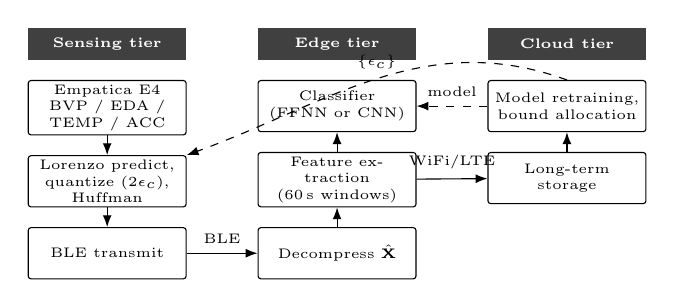
\begin{tikzpicture}[font=\scriptsize, node distance=2.5mm and 9mm, box/.style={draw, rounded corners=1pt, align=center, text width=19mm, minimum height=6.5mm, inner sep=1.5pt, font=\tiny}, tier/.style={fill=black!75, text=white, font=\tiny\bfseries, text width=19mm, align=center, minimum height=4mm, inner sep=1.5pt}, arr/.style={-{Latex[length=1.5mm]}}]
\node[tier] (t1) {Sensing tier};
\node[box, below=of t1] (e4) {Empatica E4\\BVP / EDA / TEMP / ACC};
\node[box, below=of e4] (cmp) {Lorenzo predict,\\quantize ($2\epsilon_c$), Huffman};
\node[box, below=of cmp] (ble) {BLE transmit};
\node[tier, right=of t1] (t2) {Edge tier};
\node[box, below=of t2] (nn) {Classifier\\(FFNN or CNN)};
\node[box, below=of nn] (fe) {Feature extraction\\(60\,s windows)};
\node[box, below=of fe] (dec) {Decompress $\hat{\mathbf{X}}$};
\node[tier, right=of t2] (t3) {Cloud tier};
\node[box, below=of t3] (rt) {Model retraining,\\bound allocation};
\node[box, below=of rt] (st) {Long-term storage};
\draw[arr] (e4) -- (cmp); \draw[arr] (cmp) -- (ble);
\draw[arr] (ble) -- node[above, font=\tiny]{BLE} (dec);
\draw[arr] (dec) -- (fe); \draw[arr] (fe) -- (nn);
\draw[arr] (fe) -- node[above, font=\tiny]{WiFi/LTE} (st);
\draw[arr] (st) -- (rt);
\draw[arr, dashed] (rt) -- node[above, font=\tiny]{model} (nn);
\draw[arr, dashed] (rt.north) to[out=160, in=20] node[above, font=\tiny]{$\{\epsilon_c\}$} (cmp.north east);
\end{tikzpicture}
\caption{Three-tier architecture. The device compresses with per-channel bounds $\epsilon_c$; the cloud recomputes the bounds from the retrained model and pushes them with the model update.}
\label{fig:arch}
\end{figure}

\subsection{Energy model}
For a radio whose transmit energy per window is $E_{\mathrm{tx}}$ at the uncompressed rate, compression by a ratio $\rho$ (uncompressed bits over transmitted bits) reduces the per-window transmit energy to $E^{(c)}_{\mathrm{tx}}=E_{\mathrm{tx}}/\rho$, assuming the radio duty cycle scales with payload~\cite{siekkinen2012}. The uncompressed representation is one IEEE float32 per sample, i.e.\ $168$ samples/s $\times$ 32 bits $=2.42$\,MB per hour for the four E4 channels; we also report bits per sample, which does not depend on that choice. The compressor requires one multiply-add, one division and a table lookup per sample, well within the budget of an ARM Cortex-M class core~\cite{azar2022}.

\section{Error-Bounded Codec}
\label{sec:codec}
\subsection{Closed-loop prediction and quantization}
Each channel is processed independently. For sample $i\ge3$ of a window the 1-D Lorenzo predictor~\cite{ibarria2003} extrapolates linearly from the two \emph{previously reconstructed} samples,
\begin{equation}
\tilde{x}_i = 2\hat{x}_{i-1}-\hat{x}_{i-2},
\label{eq:lorenzo}
\end{equation}
the residual $r_i=x_i-\tilde{x}_i$ is quantized to the nearest multiple of $q=2\epsilon$, $k_i=\lfloor r_i/q+\tfrac12\rfloor$, and the reconstruction is $\hat{x}_i=\tilde{x}_i+k_iq$. Because the decoder forms the identical $\tilde{x}_i$ from the same reconstructed history, $|\hat{x}_i-x_i|=|k_iq-r_i|\le q/2=\epsilon$ for every sample. The first two samples of each window are stored as quantized absolute values (32-bit indices), and any residual whose index would exceed $2^{15}-1$ is escaped and stored as a quantized absolute value, so the bound holds unconditionally (Algorithm~\ref{alg:pipe}).

The closed loop is essential. An earlier draft predicted from the \emph{original} samples $x_{i-1},x_{i-2}$; the decoder cannot form that prediction, quantization errors accumulate through the second-order recursion, and on WESAD the resulting peak error is $\minOpenLoopSci$ to $\maxOpenLoopSci$ times $\epsilon$ (Section~\ref{sec:verif}). Any evaluation of ``error-bounded'' compression must therefore verify the bound on the decoder's output, which we do for every sample.

\begin{algorithm}[t]
\caption{On-device compression of one transmit window}
\label{alg:pipe}
\begin{algorithmic}[1]
\REQUIRE window $\mathbf{X}\in\mathbb{R}^{M\times N}$, per-channel bounds $\{\epsilon_c\}$
\ENSURE bitstream $\mathbf{b}$
\FOR{each channel $c=1$ \TO $N$}
  \STATE $q\leftarrow 2\epsilon_c$; \quad $\hat{x}_1,\hat{x}_2\leftarrow q\lfloor x_{1,2}/q+\tfrac12\rfloor$ (stored)
  \FOR{$i=3$ \TO $M$}
    \STATE $\tilde{x}_i\leftarrow 2\hat{x}_{i-1}-\hat{x}_{i-2}$;\quad $k_i\leftarrow\lfloor(x_i-\tilde{x}_i)/q+\tfrac12\rfloor$
    \STATE \textbf{if} $|k_i|>2^{15}-1$ \textbf{then} escape: $\hat{x}_i\leftarrow q\lfloor x_i/q+\tfrac12\rfloor$ \textbf{else} $\hat{x}_i\leftarrow\tilde{x}_i+k_iq$
  \ENDFOR
  \STATE Huffman-encode $\{k_i\}$ with a per-window canonical table; append table and codes to $\mathbf{b}$
\ENDFOR
\RETURN $\mathbf{b}$
\end{algorithmic}
\end{algorithm}

\subsection{Entropy coding and bit accounting}
Residual indices are Huffman-coded~\cite{huffman1952} per transmit window and channel. All overheads are counted: a 16-bit length, two 32-bit boundary indices, a canonical code table (16 bits per symbol plus 6 bits per code length) and 32 bits per escaped sample. The compression ratio is total uncompressed bits over total transmitted bits across all channels, subjects and windows; this \emph{rate-weighted} ratio determines radio energy and is dominated by BVP and ACC, which carry \pctSamplesBVPACC\% of all samples.

\subsection{Scaling the bound across heterogeneous channels}
\label{sec:scale}
The four E4 channels have very different physical scales. We express the bound of channel $c$ as $\epsilon_c=\epsilon\,\sigma_c$, where $\sigma_c$ is the global standard deviation of the channel over the corpus (WESAD: BVP \sigmaBVP, EDA \sigmaEDA\,$\mu$S, TEMP \sigmaTEMP\,$^\circ$C, ACC \sigmaACC{} in units of $1/64$\,g), label-free constants stored in firmware. A \emph{uniform} bound uses the same $\epsilon$ for every channel, the natural baseline and the scheme of prior error-bounded compressors; the allocation method of Section~\ref{sec:alloc} chooses $\epsilon$ per channel.

\subsection{Baselines}
\emph{Scalar quantization} uses the same bins $q=2\epsilon_c$ without prediction, coding each window with the cheaper of fixed-length packing and Huffman coding; it is error-bounded and isolates the contribution of the predictor. \emph{Downsampling} keeps every $D$-th float32 sample ($D\in\{2,4,8\}$, ratio exactly $D$) with linear interpolation at the receiver; it has no error bound. \emph{ZFP}~\cite{lindstrom2014} runs in fixed-accuracy mode with tolerance $\epsilon_c$ on each whole per-subject channel stream, which avoids per-stream header overhead and favours the baseline; its realized worst-case error is verified like ours, since fixed-accuracy ZFP does not formally guarantee the tolerance. \emph{Lossless} coding applies zlib (level~9) to the float32 bytes. Finally, the proposed codec at the sensors' \emph{native resolution} ($\epsilon$ equal to half the sensor quantization step, exact for BVP, TEMP and ACC) gives the lossless reference point of the pipeline itself.

\section{Inference-Aware Bound Allocation}
\label{sec:alloc}
\subsection{Problem}
Let the channels be partitioned into groups $g\in\mathcal{G}$ that share a bound (here BVP, EDA, TEMP and the three ACC axes), and let $\ell_g$ index the bound level of group $g$ on a grid $\mathcal{L}=\{\epsilon^{(0)}=0<\epsilon^{(1)}<\dots<\epsilon^{(L)}\}$ expressed in units of $\sigma_g$. An allocation is a vector $\boldsymbol{\ell}=(\ell_g)_{g\in\mathcal{G}}$. For a transmission budget expressed as a target ratio $\rho_t$ we seek
\begin{equation}
\boldsymbol{\ell}^\star=\arg\min_{\boldsymbol{\ell}}\ \sum_{g} D_g(\ell_g)\quad\text{s.t.}\quad \frac{R_{\mathrm{raw}}}{\sum_g R_g(\ell_g)}\ \ge\ \rho_t,
\label{eq:alloc}
\end{equation}
where $R_g(\ell)$ is the number of bits the codec emits for group $g$ at level $\ell$ and $D_g(\ell)$ is a distortion that predicts the harm done to the inference. Both curves are measured on the training subjects of the current fold only, so the allocation is a function of training data, exactly like the classifier.

\subsection{Rate and distortion curves}
$R_g(\ell)$ is obtained by running the codec of Section~\ref{sec:codec} on the training subjects. We consider two distortion proxies.

\emph{Feature distortion} (label-free). Let $\mathbf{f}^{(0)}_w$ be the feature vector of window $w$ computed from uncompressed signals and $\mathbf{f}^{(\ell)}_{w,g}$ the same vector when only the channels of group $g$ are reconstructed at level $\ell$. With $s_j$ the standard deviation of feature $j$ over training windows,
\begin{equation}
D^{\mathrm{feat}}_g(\ell)=\frac{1}{|W|\,|J_g|}\sum_{w\in W}\sum_{j\in J_g}\left(\frac{f^{(\ell)}_{w,g,j}-f^{(0)}_{w,j}}{s_j}\right)^2,
\end{equation}
where $J_g$ is the set of features that depend on group $g$; no labels and no model are required.

\emph{Classifier distortion}. Let $h(\cdot)$ be the log-probability output of a classifier trained on uncompressed training features. Then
\begin{equation}
D^{\mathrm{clf}}_g(\ell)=\frac{1}{|W|}\sum_{w\in W}\left\|h(\mathbf{f}^{(\ell)}_{w,g})-h(\mathbf{f}^{(0)}_{w})\right\|_2^2 ,
\end{equation}
the mean squared change of the model's output when only group $g$ is compressed, which automatically discounts features the model does not use.

\subsection{Additivity and solution}
Equation~\eqref{eq:alloc} assumes that distortions add across groups: exact for $D^{\mathrm{feat}}$ because feature sets of different groups are disjoint, a first-order approximation for $D^{\mathrm{clf}}$. Because $|\mathcal{G}|=4$ and $|\mathcal{L}|=\allocNLevels$, the feasible set has $\allocNCombos$ allocations, and~\eqref{eq:alloc} is solved exactly by enumeration in milliseconds; a Lagrangian method~\cite{shoham1988} would be needed only for many more groups. The uniform baseline is solved by the same rule restricted to equal $\ell_g$, i.e.\ the smallest uniform level whose training-set ratio meets $\rho_t$, so all methods are compared under the same selection rule, and the achieved ratio on the held-out subject is reported alongside accuracy. Allocation runs in the cloud or on the edge, where the training data and the model live; the device receives $|\mathcal{G}|$ numbers with each model update and runs Algorithm~\ref{alg:pipe} unchanged.

\section{Experimental Setup}
\label{sec:setup}
\textbf{Datasets and tasks.} WESAD~\cite{schmidt2018} provides synchronized recordings of 15 subjects in baseline, stress (Trier Social Stress Test) and amusement conditions; the task is binary stress vs.\ non-stress. PPG-DaLiA~\cite{reiss2019} records 15 subjects with the same wrist device during eight daily activities for about 2.5\,h each; the task is eight-class activity recognition on the wrist channels alone, with transient periods excluded. The nurse dataset~\cite{hosseini2022} contains about 1\,250\,h of E4 recordings from 15 nurses during hospital shifts in 2020, with self-reported stress events in survey intervals; we use 60\,s windows lying entirely inside a labeled interval, binary stress (medium or high) vs.\ none, and evaluate the \nurseNSubjects{} nurses who reported both classes (training uses all \nurseNAll). Survey times are local; the UTC offset was chosen as the one that maximizes the number of survey intervals covered by a recording. In all cases only the E4 channels are used: BVP 64\,Hz, EDA 4\,Hz, TEMP 4\,Hz, ACC 32\,Hz; the scale constants $\sigma_c$ are computed per corpus.

\textbf{Windows and features.} Windows of 60\,s with a 10\,s stride are labelled by the majority label if its purity exceeds 90\%: \nWindows{} windows on WESAD (\pctStress\% stress), \daliaNWindows{} on PPG-DaLiA, \nurseNWindows{} on the nurse data (\nursePctStress\% stress, so macro-F1 is its primary metric). From each (reconstructed) window we compute \nFeatures{} standard features: BVP statistics, heart rate and heart-rate variability from band-pass-filtered BVP peaks (mean HR, SDNN, RMSSD, pNN50) and spectral power ratios; EDA statistics, slope, tonic level and skin-conductance-response count and amplitude; TEMP statistics and slope; and per-axis and magnitude statistics, jerk and spectral peak of ACC.

\textbf{Models.} The primary classifier is a feed-forward network (FFNN) with two hidden layers (64 and 32 units, ReLU, Adam, $L_2=10^{-3}$) on standardized features with random oversampling of minority classes. To test dependence on hand-crafted features, we also train a 1-D convolutional network (CNN; four strided convolution blocks, global average pooling, \cnnNParams{} parameters, \cnnEpochs{} epochs, class-weighted cross-entropy) directly on the six reconstructed waveforms at 32\,Hz, a $6\times1920$ tensor per window standardized per channel from the training fold.

\textbf{Protocol and statistics.} Evaluation is LOSO: for each subject the model is trained on the other 14 and tested on the held-out subject; FFNN results are averaged over \nSeeds{} random seeds and CNN results over \cnnNSeeds. We report mean accuracy and macro-F1 across subjects with 95\% confidence intervals, and paired differences with a Wilcoxon signed-rank test ($n=15$). For the allocation experiment, rate and distortion curves are computed inside each fold from the training subjects, the allocation is applied to the held-out subject, and the classifier is trained on training subjects compressed with the same allocation. Because the discrete grid prevents hitting a target ratio exactly, we additionally interpolate each subject's accuracy as a function of $\log\rho$ at common ratios $\rho\in\{8,\dots,24\}$ and compare methods at matched ratio, reporting the mean over that range as a summary of the operating curve.

\textbf{Bound verification.} For every error-bounded method, subject, channel and setting, the code records $\max_i|\hat{x}_i-x_i|/\epsilon_c$; it refuses to write the paper's tables if the proposed codec exceeds~1 on any sample, and reports baseline violations as results. An independent decoder must also reproduce the encoder's reconstruction bit-exactly.

\section{Results}
\label{sec:results}
\subsection{Bound verification}
\label{sec:verif}
Across all settings, subjects and channels of the three datasets the proposed codec never exceeded $\epsilon$; on WESAD the worst-case ratio $\max|\hat{x}-x|/\epsilon$ is \maxErrRatioAll{} over all $\nSamplesSci$ reconstructed samples (Table~\ref{tab:channels}), and the decoder reproduced the encoder reconstruction bit-exactly. The open-loop predictor of the earlier draft, run on the same data, exceeded $\epsilon$ by a factor of $\minOpenLoopSci$ to $\maxOpenLoopSci$.

\subsection{Uniform bound: compression--accuracy trade-off on WESAD}
\begin{table}[t]
\caption{WESAD, uniform bound: ratio and LOSO accuracy of the proposed codec (matched; mean $\pm$ 95\% CI over 15 subjects; $p$: Wilcoxon vs.\ uncompressed).}
\label{tab:main}
\centering\scriptsize
\resizebox{\columnwidth}{!}{\begin{tabular}{lccccccc}
\toprule
Config. & $\epsilon/\sigma$ & Ratio $\rho$ & bits/samp. & Acc. (\%) & $\Delta$Acc. & $p$ & F1 (\%) \\
\midrule
Uncompressed & --- & 1.0$\times$ & 32.00 & 89.4 $\pm$ 5.3 & --- & --- & 86.6 \\
Proposed & 0.005 & 8.8$\times$ & 3.63 & 89.3 $\pm$ 5.0 & -0.1 & 0.73 & 86.7 \\
Proposed & 0.01 & 10.5$\times$ & 3.04 & 89.2 $\pm$ 5.1 & -0.1 & 0.78 & 86.7 \\
Proposed & 0.02 & 13.3$\times$ & 2.41 & 89.9 $\pm$ 4.9 & +0.6 & 0.20 & 87.2 \\
Proposed & 0.05 & 17.5$\times$ & 1.83 & 90.8 $\pm$ 4.5 & +1.5 & 0.07 & 88.3 \\
Proposed & 0.1 & 20.6$\times$ & 1.55 & 89.5 $\pm$ 4.1 & +0.1 & 0.44 & 86.6 \\
Proposed & 0.2 & 23.6$\times$ & 1.35 & 87.9 $\pm$ 4.9 & -1.4 & 0.30 & 84.8 \\
\bottomrule
\end{tabular}
}
\end{table}
\begin{table}[t]
\caption{WESAD baselines. Top: error-bounded methods at each uniform $\epsilon$ (ratio, accuracy change in points, realized worst-case error for ZFP). Bottom: methods without a tunable bound (ratio, matched $\Delta$Acc., mismatched accuracy).}
\label{tab:baselines}
\centering\scriptsize
\resizebox{\columnwidth}{!}{\begin{tabular}{lcccccc}
\toprule
$\epsilon/\sigma$ & 0.005 & 0.01 & 0.02 & 0.05 & 0.1 & 0.2 \\
\midrule
Proposed: ratio $\rho$ & 8.8$\times$ & 10.5$\times$ & 13.3$\times$ & 17.5$\times$ & 20.6$\times$ & 23.6$\times$ \\
Proposed: $\Delta$Acc. & -0.1 & -0.1 & +0.6 & +1.5 & +0.1 & -1.4 \\
Scalar quant.: ratio $\rho$ & 5.1$\times$ & 5.5$\times$ & 6.6$\times$ & 9.3$\times$ & 12.1$\times$ & 16.0$\times$ \\
Scalar quant.: $\Delta$Acc. & -0.1 & -0.1 & +0.6 & +1.5 & +0.1 & -1.5 \\
ZFP: ratio $\rho$ & 3.1$\times$ & 3.4$\times$ & 3.7$\times$ & 4.2$\times$ & 4.7$\times$ & 5.3$\times$ \\
ZFP: realized $\max|\hat{x}-x|/\epsilon$ & 0.47 & 0.47 & 0.57 & 0.46 & 0.46 & 0.46 \\
ZFP: $\Delta$Acc. & -0.0 & +0.5 & +0.1 & +1.6 & +0.7 & +1.0 \\
\midrule
\multicolumn{7}{l}{\emph{Not error-bounded / reference:} ratio, $\Delta$Acc. matched, Acc. mismatched} \\
Downsampling $D=2$ & \multicolumn{6}{l}{2.0$\times$, +0.6, 88.7\%} \\
Downsampling $D=4$ & \multicolumn{6}{l}{4.0$\times$, +2.6, 86.9\%} \\
Downsampling $D=8$ & \multicolumn{6}{l}{8.0$\times$, +3.6, 84.8\%} \\
Lossless zlib & \multicolumn{6}{l}{3.2$\times$, -0.0, 89.4\%} \\
Proposed, native resolution & \multicolumn{6}{l}{4.6$\times$, +0.0, 89.4\%} \\
\bottomrule
\end{tabular}
}
\end{table}
\begin{table}[t]
\caption{WESAD: per-channel ratio at each uniform bound and worst-case $\max|\hat{x}-x|/\epsilon$ over all subjects and samples.}
\label{tab:channels}
\centering\scriptsize
\resizebox{\columnwidth}{!}{\begin{tabular}{lccccccc}
\toprule
Channel & $\sigma$ (unit) & $\epsilon=0.005\sigma$ & $\epsilon=0.01\sigma$ & $\epsilon=0.02\sigma$ & $\epsilon=0.05\sigma$ & $\epsilon=0.1\sigma$ & $\epsilon=0.2\sigma$ \\
\midrule
BVP & 65.2 a.u. & 9.4$\times$ & 11.9$\times$ & 14.4$\times$ & 17.5$\times$ & 20.0$\times$ & 22.7$\times$ \\
EDA & 2.34 $\mu$S & 11.6$\times$ & 13.9$\times$ & 16.1$\times$ & 18.3$\times$ & 19.5$\times$ & 20.2$\times$ \\
TEMP & 1.5 $^\circ$C & 11.8$\times$ & 15.1$\times$ & 18.0$\times$ & 19.2$\times$ & 20.1$\times$ & 20.9$\times$ \\
ACC x & 35.7 1/64\,g & 7.4$\times$ & 8.6$\times$ & 11.1$\times$ & 15.9$\times$ & 19.7$\times$ & 23.5$\times$ \\
ACC y & 35.7 1/64\,g & 10.0$\times$ & 11.3$\times$ & 14.7$\times$ & 20.0$\times$ & 23.3$\times$ & 26.0$\times$ \\
ACC z & 35.7 1/64\,g & 7.9$\times$ & 9.2$\times$ & 12.0$\times$ & 16.9$\times$ & 20.8$\times$ & 24.3$\times$ \\
\midrule
All (rate-weighted) & & 8.8$\times$ & 10.5$\times$ & 13.3$\times$ & 17.5$\times$ & 20.6$\times$ & 23.6$\times$ \\
Max $|\hat{x}-x|/\epsilon$ & & 1.000 & 1.000 & 1.000 & 1.000 & 1.000 & 1.000 \\
\bottomrule
\end{tabular}
}
\end{table}

Table~\ref{tab:main} shows the uncompressed FFNN at \rawAcc\% accuracy (macro-F1 \rawF\%), within the range reported for wrist-only WESAD classifiers~\cite{sipele2023}. From $\epsilon=0.005\sigma$ to $0.1\sigma$ the ratio grows from \ratioEa$\times$ to \ratioEe$\times$ while no paired accuracy difference is significant (changes of \dAccEa{} to +\dAccEe{} points, smallest $p=\pAccEd$); only at $0.2\sigma$ (\ratioEf$\times$) does accuracy fall, by \dAccEf{} points ($p=\pAccEf$, not significant with 15 subjects). The stress classifier therefore tolerates a reconstruction error of a tenth of a standard deviation on every channel, a $20\times$ reduction in payload, without measurable loss. Per channel (Table~\ref{tab:channels}) the smooth, oversampled TEMP and EDA streams compress most at tight bounds, and at loose bounds every channel approaches the one-bit-per-sample floor of Huffman coding.

\subsection{Baselines}
Table~\ref{tab:baselines} isolates the contributions. Scalar quantization reconstructs onto the same grid and reaches the same accuracy as the proposed codec at every $\epsilon$, so the Lorenzo predictor costs nothing in fidelity and multiplies the ratio by \predGainMin$\times$ to \predGainMax$\times$. ZFP in fixed-accuracy mode realizes only \zfpErrMin{} to \zfpErrMax{} of the permitted error and reaches \zfpRatioMin$\times$ to \zfpRatioMax$\times$ even with whole-stream encoding; its accuracy changes (\zfpDAccMin{} to \zfpDAccMax{} points) reflect that smaller realized error. Downsampling with retraining does something unexpected on WESAD: it \emph{improves} accuracy, to \dsAccC\% at $D=4$ (\dsDAccC{} points, $p=\dsPC$) and \dsAccE\% at $D=8$ (\dsDAccE{} points, $p=\dsPE$), because linear interpolation low-pass filters the accelerometer and pulse channels and the smoothed features generalize better across subjects; the codec, which preserves the signal to within $\epsilon$, cannot produce such a gain by design. Downsampling, however, offers no reconstruction guarantee, cannot go beyond $8\times$ without discarding the pulse waveform, and, as shown below, fails when the model is not retrained. The codec reaches \ratioEe$\times$ at \dAccEe{} points, two and a half times the ratio of the best downsampling setting. Lossless zlib gives \ratioLossless$\times$; the codec at native resolution gives \ratioNative$\times$ at \accNative\%.

\subsection{Inference-aware allocation on WESAD}
\begin{figure}[t]
\centering
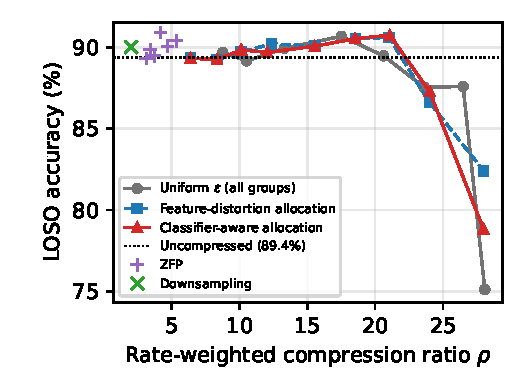
\includegraphics[width=0.9\columnwidth]{results_alloc/fig_pareto.pdf}
\caption{WESAD: LOSO accuracy vs.\ achieved rate-weighted ratio for the uniform bound and the two allocation methods (each point is one target $\rho_t$; mean over 15 subjects and \nSeeds{} seeds), with downsampling and ZFP for reference.}
\label{fig:pareto}
\end{figure}
\begin{figure}[t]
\centering
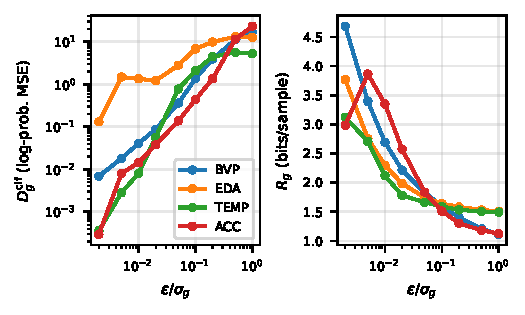
\includegraphics[width=0.9\columnwidth]{results_alloc/fig_curves.pdf}
\caption{WESAD: classifier distortion $D^{\mathrm{clf}}_g$ (left) and rate $R_g$ (right) per channel group vs.\ the bound, averaged over the 15 training folds. EDA and TEMP are cheap to transmit but sensitive to the bound; ACC and BVP dominate the rate.}
\label{fig:curves}
\end{figure}
\begin{table}[t]
\caption{WESAD: accuracy at matched ratio (per-subject interpolation; mean over 15 subjects) and Wilcoxon $p$ of each allocation vs.\ the uniform bound.}
\label{tab:matched}
\centering\scriptsize
\resizebox{\columnwidth}{!}{\begin{tabular}{lccccccccc}
\toprule
Method & $\rho=8$ & $\rho=10$ & $\rho=12$ & $\rho=14$ & $\rho=16$ & $\rho=18$ & $\rho=20$ & $\rho=22$ & $\rho=24$ \\
\midrule
Uniform $\epsilon$ & 91.2 & 89.4 & 89.4 & 90.1 & 90.5 & 90.2 & 89.4 & 89.1 & 87.4 \\
Feature-distortion alloc. & 89.3 & 89.5 & 90.3 & 90.2 & 90.0 & 90.2 & 90.5 & 90.1 & 87.3 \\
Classifier-aware alloc. & 89.2 & 89.7 & 89.8 & 90.0 & 90.0 & 90.3 & 90.7 & 90.4 & 87.7 \\
\quad $p$ (Feature-distortion vs.\ uniform) & 0.25 & 0.55 & 0.08 & 0.92 & 0.27 & 0.56 & 0.19 & 0.28 & 0.93 \\
\quad $p$ (Classifier-aware vs.\ uniform) & 0.50 & 0.27 & 0.16 & 0.47 & 0.16 & 0.39 & 0.11 & 0.23 & 0.68 \\
\bottomrule
\end{tabular}
}
\end{table}
\begin{table}[t]
\caption{WESAD: median bound level $\epsilon_g/\sigma_g$ chosen by the classifier-aware allocation per target ratio.}
\label{tab:levels}
\centering\scriptsize
\begin{tabular}{ccccc}
\toprule
Target $\rho_t$ & BVP & EDA & TEMP & ACC \\
\midrule
$\ge4$ & 0.002 & 0 & 0 & 0.002 \\
$\ge6$ & 0.002 & 0 & 0 & 0.002 \\
$\ge8$ & 0.005 & 0 & 0.002 & 0.002 \\
$\ge10$ & 0.02 & 0 & 0.002 & 0.02 \\
$\ge12$ & 0.01 & 0.002 & 0.002 & 0.02 \\
$\ge15$ & 0.02 & 0.002 & 0.002 & 0.05 \\
$\ge18$ & 0.05 & 0.002 & 0.002 & 0.1 \\
$\ge21$ & 0.1 & 0.002 & 0.002 & 0.2 \\
$\ge24$ & 0.5 & 0.002 & 0.01 & 0.2 \\
$\ge28$ & 1 & 0.1 & 1 & 1 \\
\bottomrule
\end{tabular}

\end{table}

Fig.~\ref{fig:pareto} shows the operating curves. Because the uniform bound is already flat to about $20\times$ on this task, there is little for the allocator to gain below that ratio: at matched ratios between $10\times$ and $18\times$ the three curves lie within one point of each other (Table~\ref{tab:matched}), averaged over $8\le\rho\le24$ the classifier-aware allocation adds only \allocAUCDiffClf{} points ($p=\allocAUCPClf$), and pooled over all targets and subjects the gain is \allocPooledDiff{} points ($p=\allocPooledP$, $n=150$). The gain appears exactly where the uniform bound begins to fail: at $\rho_t\ge21$ the uniform scheme reaches \allocUniformRatioBA$\times$ at \allocUniformAccBA\% while the allocation reaches \allocClfRatioBA$\times$ at \allocClfAccBA\%, a paired difference of \allocClfDiffBA{} points ($p=\allocClfPBA$); at matched $\rho=20$ the difference is \allocMatchedDiffClfBZ{} points ($p=\allocMatchedPClfBZ$). At $\rho_t\ge24$ all schemes have exhausted the cheap channels and the difference vanishes. Table~\ref{tab:levels} shows what the allocator does: it keeps EDA and TEMP at the tightest levels and spends the budget on ACC and BVP, the pattern suggested by the curves of Fig.~\ref{fig:curves}. That the label-free proxy tracks the classifier-aware one means the allocation can be computed without labels or a trained model, from the feature extractor alone.

\subsection{Generalization: activity recognition on PPG-DaLiA}
\begin{table}[t]
\caption{PPG-DaLiA, eight-class activity recognition from the wrist channels (LOSO, 15 subjects, \nSeeds{} seeds, matched scenario).}
\label{tab:dalia}
\centering\scriptsize
\resizebox{\columnwidth}{!}{\begin{tabular}{llcccccc}
\toprule
Method & Setting & Ratio $\rho$ & Acc. (\%) & $\Delta$Acc. & $p$ & F1 (\%) & $\Delta$F1 \\
\midrule
Uncompressed & --- & 1.0$\times$ & 70.6 $\pm$ 8.4 & --- & --- & 72.3 & --- \\
Proposed & $\epsilon=0.005\sigma$ & 5.7$\times$ & 70.7 $\pm$ 8.3 & +0.1 & 0.64 & 72.1 & -0.2 \\
Proposed & $\epsilon=0.01\sigma$ & 7.2$\times$ & 70.4 $\pm$ 8.5 & -0.2 & 0.28 & 72.6 & +0.3 \\
Proposed & $\epsilon=0.02\sigma$ & 9.2$\times$ & 70.5 $\pm$ 8.3 & -0.1 & 0.93 & 72.3 & -0.1 \\
Proposed & $\epsilon=0.05\sigma$ & 12.5$\times$ & 70.1 $\pm$ 8.2 & -0.5 & 0.33 & 72.0 & -0.4 \\
Proposed & $\epsilon=0.1\sigma$ & 15.4$\times$ & 70.3 $\pm$ 8.9 & -0.2 & 0.72 & 72.4 & +0.0 \\
Proposed & $\epsilon=0.2\sigma$ & 18.6$\times$ & 68.9 $\pm$ 8.8 & -1.7 & 0.21 & 71.8 & -0.5 \\
Downsampling & $D=2$ & 2.0$\times$ & 69.8 $\pm$ 8.4 & -0.8 & 0.12 & 71.3 & -1.0 \\
Downsampling & $D=4$ & 4.0$\times$ & 69.9 $\pm$ 8.8 & -0.7 & 0.25 & 71.9 & -0.4 \\
Downsampling & $D=8$ & 8.0$\times$ & 67.8 $\pm$ 8.5 & -2.8 & $<$0.01 & 69.9 & -2.5 \\
Lossless zlib & --- & 2.6$\times$ & 70.6 $\pm$ 8.4 & +0.0 & 1.00 & 72.3 & +0.0 \\
\bottomrule
\end{tabular}
}
\end{table}
\begin{figure}[t]
\centering
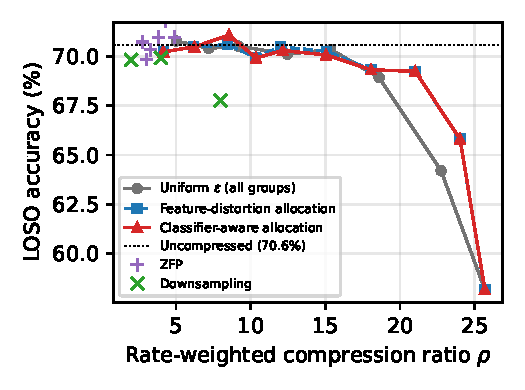
\includegraphics[width=0.9\columnwidth]{results_alloc_dalia/fig_pareto.pdf}
\caption{PPG-DaLiA: LOSO accuracy vs.\ achieved ratio for the uniform bound and the two allocation methods.}
\label{fig:pareto_dalia}
\end{figure}
Table~\ref{tab:dalia} reports the eight-class activity task. The uncompressed FFNN reaches \daliaRawAcc\% accuracy (macro-F1 \daliaRawF\%) from the wrist channels alone, a harder problem than binary stress detection. The codec behaves as on WESAD: from $\epsilon=0.005\sigma$ (\daliaRatioEa$\times$, \daliaDAccEa{} points) to $0.1\sigma$ (\daliaRatioEe$\times$, \daliaDAccEe{} points, $p=\daliaPEe$) no accuracy change is significant, and $0.2\sigma$ gives \daliaRatioEf$\times$ at \daliaDAccEf{} points ($p=\daliaPEf$). Downsampling is weaker on this task than on WESAD: $D=8$ costs \daliaDsDAccH{} points ($p\daliaDsPrelH$), significantly worse than the codec at nearly twice the ratio. ZFP again realizes only \daliaZfpErrMin{} to \daliaZfpErrMax{} of the permitted error and reaches at most \daliaZfpRatioMax$\times$. Fig.~\ref{fig:pareto_dalia} shows the allocation experiment, with all curves, bounds and scale constants recomputed for the new corpus. The pattern of WESAD repeats: up to about $18\times$ the uniform bound and the allocations are indistinguishable; beyond that the uniform curve collapses while the allocated curves degrade gracefully, giving \daliaallocClfDiffBA{} points at \daliaallocClfRatioBA$\times$ ($p=\daliaallocClfPBA$) and \daliaallocClfDiffBD{} points at \daliaallocClfRatioBD$\times$ ($p=\daliaallocClfPBD$). Pooled over all targets and subjects the paired gain is \daliaallocPooledDiff{} points ($p=\daliaallocPooledP$, $n=150$); averaged over $8\le\rho\le24$ it is \daliaallocAUCDiffClf{} points, which does not reach significance ($p=\daliaallocAUCPClf$) because the gain is concentrated at the high-ratio end. The allocator again keeps EDA and TEMP tight and loosens ACC and BVP, and the label-free proxy again matches the classifier-aware one (\daliaallocAUCDiffFeat{} points). The method therefore transfers to a different task, label space and corpus without any change.

\subsection{Generalization: in-the-wild nurse stress}
\begin{table}[t]
\caption{Nurse stress (in the wild): self-reported stress vs.\ none, LOSO over \nurseNSubjects{} nurses, \nSeeds{} seeds. F1 is macro-F1; ``F1 mism.''\ is an uncompressed-trained model on reconstructed data.}
\label{tab:nurse}
\centering\scriptsize
\resizebox{\columnwidth}{!}{\begin{tabular}{llcccccc}
\toprule
Method & Setting & Ratio $\rho$ & Acc. (\%) & F1 (\%) & $\Delta$F1 & $p$ & F1 mism. (\%) \\
\midrule
Uncompressed & --- & 1.0$\times$ & 67.4 & 48.6 $\pm$ 5.0 & --- & --- & 48.6 \\
Proposed & $\epsilon=0.005\sigma$ & 6.4$\times$ & 67.8 & 48.7 $\pm$ 5.2 & +0.1 & 0.68 & 48.5 \\
Proposed & $\epsilon=0.01\sigma$ & 7.9$\times$ & 66.7 & 48.3 $\pm$ 5.2 & -0.3 & 0.64 & 48.2 \\
Proposed & $\epsilon=0.02\sigma$ & 10.2$\times$ & 67.7 & 49.1 $\pm$ 5.4 & +0.6 & 0.38 & 48.8 \\
Proposed & $\epsilon=0.05\sigma$ & 14.0$\times$ & 67.6 & 49.0 $\pm$ 4.9 & +0.4 & 0.79 & 47.5 \\
Proposed & $\epsilon=0.1\sigma$ & 17.4$\times$ & 66.5 & 48.1 $\pm$ 5.9 & -0.5 & 0.45 & 46.9 \\
Proposed & $\epsilon=0.2\sigma$ & 20.8$\times$ & 66.3 & 48.2 $\pm$ 5.9 & -0.4 & 0.54 & 45.8 \\
Downsampling & $D=2$ & 2.0$\times$ & 67.9 & 48.8 $\pm$ 5.1 & +0.3 & 0.50 & 47.9 \\
Downsampling & $D=4$ & 4.0$\times$ & 67.4 & 48.3 $\pm$ 5.3 & -0.3 & 0.41 & 47.6 \\
Downsampling & $D=8$ & 8.0$\times$ & 67.0 & 47.8 $\pm$ 4.9 & -0.7 & 0.22 & 46.7 \\
Lossless zlib & --- & 2.8$\times$ & 67.4 & 48.6 $\pm$ 5.0 & +0.0 & 1.00 & 48.6 \\
\bottomrule
\end{tabular}
}
\end{table}
Table~\ref{tab:nurse} reports the hardest and least controlled task. Self-reported stress during real hospital shifts, with survey intervals of minutes to an hour and \nursePctStress\% of labeled windows marked as stress, is barely detectable from the wrist with this feature set: the uncompressed FFNN reaches a macro-F1 of \nurseRawF\% (accuracy \nurseRawAcc\%), close to chance, in line with the modest results reported for this dataset. Its purpose here is to test whether compression changes whatever the model does detect, on in-the-wild data with motion artefacts, sensor detachment and long unlabeled stretches. It does not: from $6\times$ to \nurseRatioEf$\times$ every change in macro-F1 is within one point (\nurseDFEd{} at \nurseRatioEd$\times$, $p=\nursePFEd$; \nurseDFEf{} at \nurseRatioEf$\times$) and none is significant, and the same holds for downsampling (\nurseDsDFH{} at $D=8$, $p=\nurseDsPFH$) and for the mismatched scenario (\nurseFMMEd\% vs.\ \nurseDsFMMH\%). Allocation accordingly has nothing to improve on a flat curve (\nurseallocPooledDiff{} points pooled, $p=\nurseallocPooledP$). A null effect on a near-chance classifier is weak evidence by itself; its value is that the codec behaves no differently on a hospital floor than in the laboratory. Notably, on this data ZFP in fixed-accuracy mode exceeded its nominal tolerance at $\epsilon=\nurseZfpErrMaxEps\sigma$ (realized \nurseZfpErrMax\,$\epsilon$), confirming that its tolerance is a target rather than a guarantee, whereas the proposed codec stayed within $\epsilon$ on every sample.

\subsection{A model without hand-crafted features}
\begin{table}[t]
\caption{WESAD, 1-D CNN on raw reconstructed waveforms (LOSO, 15 subjects, \cnnNSeeds{} seeds).}
\label{tab:cnn}
\centering\scriptsize
\resizebox{\columnwidth}{!}{\begin{tabular}{lcccccc}
\toprule
Config. & Ratio $\rho$ & Acc. (\%) & $\Delta$Acc. & $p$ & F1 (\%) & Acc. mismatched (\%) \\
\midrule
Uncompressed & 1.0$\times$ & 89.9 $\pm$ 3.8 & --- & --- & 87.4 & 89.9 \\
Proposed $\epsilon=0.01\sigma$ & 10.5$\times$ & 87.7 $\pm$ 3.8 & -2.2 & 0.01 & 85.4 & 88.6 \\
Proposed $\epsilon=0.02\sigma$ & 13.3$\times$ & 89.2 $\pm$ 3.5 & -0.7 & 0.36 & 86.7 & 87.6 \\
Proposed $\epsilon=0.05\sigma$ & 17.5$\times$ & 89.5 $\pm$ 3.7 & -0.4 & 0.25 & 87.0 & 87.2 \\
Proposed $\epsilon=0.1\sigma$ & 20.6$\times$ & 87.1 $\pm$ 4.4 & -2.7 & 0.06 & 84.2 & 86.2 \\
Proposed $\epsilon=0.2\sigma$ & 23.6$\times$ & 89.3 $\pm$ 4.0 & -0.5 & 1.00 & 86.7 & 83.5 \\
Downsampling $D=4$ & 4.0$\times$ & 87.7 $\pm$ 4.0 & -2.2 & 0.05 & 85.5 & 87.4 \\
Downsampling $D=8$ & 8.0$\times$ & 87.3 $\pm$ 4.0 & -2.6 & 0.01 & 84.3 & 86.5 \\
\bottomrule
\end{tabular}
}
\end{table}
Table~\ref{tab:cnn} repeats the WESAD experiment with the CNN, which sees the reconstructed waveforms directly rather than through the feature extractor. It reaches \cnnRawAcc\% uncompressed (macro-F1 \cnnRawF\%), on par with the FFNN. Its response to compression is noisier and not monotonic in $\epsilon$: \cnnDAccEb{} points at \ratioEb$\times$ ($p=\cnnPEb$), \cnnDAccEd{} at \ratioEd$\times$ ($p=\cnnPEd$), \cnnDAccEe{} at \ratioEe$\times$ ($p=\cnnPEe$) and \cnnDAccEf{} at \ratioEf$\times$ ($p=\cnnPEf$). Differences of this size are within the seed-to-seed variation, so the fair reading is that the CNN tolerates all tested bounds to within about three points with no systematic trend. Downsampling, in contrast, hurts the CNN consistently (\cnnDsDAccD{} points at $D=4$, \cnnDsDAccH{} at $D=8$, $p\le0.05$), the opposite of its effect on the FFNN: a model that reads the waveform does not benefit from the smoothing that helped the hand-crafted features.

\begin{table}[t]
\caption{WESAD: allocations chosen with the feature pipeline evaluated with the CNN (LOSO, \cnnallocNSeeds{} seeds, \cnnallocEpochs{} epochs).}
\label{tab:cnnalloc}
\centering\scriptsize
\resizebox{\columnwidth}{!}{\begin{tabular}{llcccc}
\toprule
Target $\rho_t$ & Method & $\rho$ & CNN Acc. (\%) & $\Delta$ vs.\ uniform & $p$ \\
\midrule
$\ge18$ & Uniform $\epsilon$ & 20.6$\times$ & 88.4 $\pm$ 3.3 & --- & --- \\
$\ge18$ & Feature-distortion alloc. & 18.5$\times$ & 88.9 $\pm$ 3.7 & +0.4 & 0.93 \\
$\ge18$ & Classifier-aware alloc. (FFNN) & 18.5$\times$ & 88.9 $\pm$ 3.7 & +0.4 & 0.93 \\
$\ge24$ & Uniform $\epsilon$ & 26.5$\times$ & 82.7 $\pm$ 5.7 & --- & --- \\
$\ge24$ & Feature-distortion alloc. & 24.0$\times$ & 81.4 $\pm$ 5.2 & -1.3 & 0.42 \\
$\ge24$ & Classifier-aware alloc. (FFNN) & 24.0$\times$ & 80.2 $\pm$ 5.5 & -2.5 & 0.14 \\
\bottomrule
\end{tabular}
}
\end{table}
\textbf{Does the allocation transfer across models?} The allocations of Section~\ref{sec:alloc} were chosen with the feature extractor and the FFNN. Table~\ref{tab:cnnalloc} applies exactly those per-fold allocations to the CNN. They do not transfer: at $\rho_t\ge18$ the label-free allocation changes CNN accuracy by \cnnallocFeatDiffAH{} points relative to the uniform bound ($p=\cnnallocFeatPAH$) and at $\rho_t\ge24$ by \cnnallocFeatDiffBD{} points ($p=\cnnallocFeatPBD$); pooled over both targets the differences are \cnnallocFeatPooledDiff{} and \cnnallocClfPooledDiff{} points ($p=\cnnallocFeatPooledP$, $p=\cnnallocClfPooledP$), i.e.\ no gain and no significant loss. This is the expected consequence of what the allocation optimizes: a distortion of the \emph{feature extractor} or of the \emph{FFNN}, neither of which the CNN uses. For a waveform model the distortion curves must be measured with that model, which the same code supports; we leave that run to future work because of its cost. The negative result delimits the claim: allocation improves the model it was computed for, not any model.

\subsection{Mismatched deployment}
When the FFNN is trained on uncompressed WESAD data and deployed on reconstructed signals, accuracy is \accMMEd\% at $\epsilon=0.05\sigma$ (matched: \accEd\%) and \accMMEe\% at $0.1\sigma$, so a model need not be retrained for bounds up to $0.05\sigma$. Downsampling behaves differently: the same model drops to \dsAccMMC\% at $D=4$ and \dsAccMME\% at $D=8$, because interpolation shifts the feature distribution in a way that bounded quantization error does not. On PPG-DaLiA the contrast is sharper: an uncompressed-trained model keeps \daliaAccMMEd\% at $\epsilon=0.05\sigma$ (\daliaRatioEd$\times$) but falls to \daliaDsAccMMH\% with $D=8$ downsampling (\daliaRawAcc\% uncompressed). For the CNN, trained uncompressed, accuracy is \cnnAccMMEd\% at $\epsilon=0.05\sigma$ and \cnnAccMMEe\% at $0.1\sigma$ against \cnnRawAcc\% uncompressed, and \cnnDsAccMMH\% for $D=8$ downsampling. Bounded quantization error is thus far more benign to a deployed model than resampling, which matters whenever retraining on compressed data is impractical.

\subsection{Device implementation}
To substantiate the on-device claim without hardware we implemented the encoder (Algorithm~\ref{alg:pipe}, including the per-window canonical Huffman table) in portable C with single-precision arithmetic, as it would run on a Cortex-M4F. First, the C encoder was run natively on \fwTestWindows{} transmit windows ($\fwTestSamplesSci$ samples) of two WESAD subjects at three bounds and compared with the double-precision reference codec: the compressed size agrees to \fwBitsRelDiff\%, the worst-case error is \fwMaxErr\,$\epsilon$ (the excess over 1 is single-precision rounding), the C decoder reproduces the C encoder exactly, and \fwIdentical\% of quantization indices are identical, the remainder differing where float32 rounding flips a bin decision and the closed loop then follows a different but equally valid path. Second, the encoder was cross-compiled (GCC~13.3, \texttt{-O2}, hard-float) and executed on an emulated Cortex-M4 (Unicorn engine) on one 60\,s window of all six channels (\fwWindowSamples{} samples): \fwInstrPerSample{} instructions per sample including Huffman table construction and bit packing, with \fwCodeKB\,KB of code and \fwRamKB\,KB of scratch RAM (unoptimized). At 64\,MHz and one instruction per cycle this is \fwTimeMs\,ms of compute per 60\,s window, a duty cycle of \fwDuty\%, and with the nRF52840 datasheet figure of 52\,$\mu$A/MHz~\cite{nrf52840} at 3\,V about \fwEnergyMJ\,mJ per window. These are estimates with stated assumptions, not measurements; they place the encoder's cost far below that of transmitting the uncompressed window over BLE~\cite{siekkinen2012}, but a measurement on hardware remains future work.

\subsection{Energy}
By the energy model, the uniform bound $\epsilon=0.1\sigma$ cuts transmit energy and hourly payload by \savingEe\% (\bpsEe{} bits per sample instead of 32) with no measurable accuracy loss on WESAD, and the allocation at \allocClfRatioBA$\times$ by \allocClfSavingBA\%; lossless coding saves only \savingLossless\%.

\section{Discussion and Limitations}
\textbf{What the guarantee is and is not.} The $\ell_\infty$ bound is on reconstruction error and is verified on every sample; the effect on classification is measured empirically and depends on the features and the model. That the label-free proxy performs as well as the classifier-aware one suggests that for these tasks the harm done by compression is dominated by feature distortion rather than by decision-boundary geometry.

\textbf{Why uniform bounds fail first on EDA.} Corpus-level scaling is coarse for EDA, whose per-subject range on WESAD varies from \minEDARange{} to \maxEDARange\,$\mu$S; at $\epsilon=0.2\sigma$ (\epsEDAEf\,$\mu$S) the EDA of low-conductance subjects collapses onto a few levels, the most likely cause of the accuracy drop at that setting; the allocator discovers this from training data and keeps EDA tight at almost no cost in rate (Table~\ref{tab:levels}). Per-subject scale estimation from a calibration period is an obvious refinement.

\textbf{Downsampling.} On WESAD, downsampling with retraining raised FFNN accuracy above the uncompressed baseline, because interpolation low-pass filters the motion and pulse channels and the smoothed features generalize better across subjects; on PPG-DaLiA, whose task depends on motion detail, the same operation significantly hurt. This is a property of the task and the features, not of the compressor: a practitioner who can retrain and whose task tolerates smoothing may prefer downsampling up to $8\times$, whereas the error-bounded codec is the choice when a guarantee, a higher ratio, or deployment without retraining is needed.

\textbf{What allocation does and does not do.} Allocation helps exactly where the uniform bound starts to hurt the model it was computed for, and nowhere else: on WESAD beyond $20\times$, on PPG-DaLiA beyond $18\times$, and for the CNN, whose distortion curves were never measured, not at all. Its value is greatest near the edge of the usable range, and it must be recomputed whenever the model changes, which the architecture of Fig.~\ref{fig:arch} accommodates.

\textbf{Statistical power and scope.} Fifteen subjects per dataset give wide confidence intervals; differences inside them should not be over-interpreted, and we report every paired $p$-value rather than only the favourable ones. Transmit energy is modelled as proportional to payload, ignoring BLE connection overhead; encoder cost is characterized by instruction counts on an emulated core and a datasheet current figure rather than by measurement; and the nurse-dataset labels are self-reports with coarse timing, so its role here is only to test whether compression changes what the model detects.

\section{Conclusion}
We presented a closed-loop, error-bounded codec for wearable physiological signals, verified its guarantee on every sample of three public datasets, and introduced inference-aware bound allocation. On WESAD the uniform bound already gives \ratioEe$\times$ compression with no significant loss in LOSO accuracy; allocation adds \allocClfDiffBA{} points where that bound starts to fail, and \daliaallocClfDiffBA{} to \daliaallocClfDiffBD{} points at $21$--$24\times$ on PPG-DaLiA, with a label-free variant performing equally well. Bounded quantization is far more benign than downsampling to a model deployed without retraining, and an allocation computed for one model does not transfer to a different model family, so the distortion curves must be measured with the model that will be deployed. The bounds are a small set of interpretable numbers that the cloud can recompute with each model update, linking radio energy to inference fidelity. Code and all result files are released with the paper.

\begin{thebibliography}{00}
\bibitem{shi2016} W. Shi \emph{et al.}, ``Edge computing: Vision and challenges,'' \emph{IEEE Internet of Things Journal}, vol. 3, no. 5, pp. 637--646, 2016.
\bibitem{zhou2019} Z. Zhou \emph{et al.}, ``Edge intelligence: Paving the last mile of artificial intelligence with edge computing,'' \emph{Proc. IEEE}, vol. 107, no. 8, pp. 1738--1762, 2019.
\bibitem{anastasi2009} G. Anastasi \emph{et al.}, ``Energy conservation in wireless sensor networks: A survey,'' \emph{Ad Hoc Networks}, vol. 7, no. 3, pp. 537--568, 2009.
\bibitem{siekkinen2012} M. Siekkinen, M. Hiienkari, J. K. Nurminen, and J. Nieminen, ``How low energy is Bluetooth Low Energy? Comparative measurements with ZigBee/802.15.4,'' in \emph{Proc. IEEE WCNC Workshops}, 2012, pp. 232--237.
\bibitem{razzaque2013} M. A. Razzaque \emph{et al.}, ``Compression in wireless sensor networks: A survey,'' \emph{ACM Trans. Sensor Networks}, vol. 10, no. 1, 2013.
\bibitem{jalaleddine1990} S. M. S. Jalaleddine, C. G. Hutchens, R. D. Strattan, and W. A. Coberly, ``ECG data compression techniques---a unified approach,'' \emph{IEEE Trans. Biomed. Eng.}, vol. 37, no. 4, pp. 329--343, 1990.
\bibitem{ramakrishnan1997} A. G. Ramakrishnan and S. Saha, ``ECG coding by wavelet-based linear prediction,'' \emph{IEEE Trans. Biomed. Eng.}, vol. 44, no. 12, 1997.
\bibitem{li2018} H. Li \emph{et al.}, ``Learning IoT in edge: Deep learning for the Internet of Things,'' \emph{IEEE Network}, vol. 32, no. 1, 2018.
\bibitem{di2016} S. Di and F. Cappello, ``Fast error-bounded lossy HPC data compression with SZ,'' in \emph{Proc. IEEE IPDPS}, 2016.
\bibitem{tao2017} D. Tao \emph{et al.}, ``Significantly improving lossy compression for scientific data sets,'' in \emph{Proc. IEEE IPDPS}, 2017.
\bibitem{liang2018} X. Liang, S. Di, D. Tao, \emph{et al.}, ``Error-controlled lossy compression optimized for high compression ratios of scientific datasets,'' in \emph{Proc. IEEE Int. Conf. Big Data}, 2018, pp. 438--447.
\bibitem{lindstrom2014} P. Lindstrom, ``Fixed-rate compressed floating-point arrays,'' \emph{IEEE Trans. Vis. Comput. Graph.}, vol. 20, no. 12, pp. 2674--2683, 2014.
\bibitem{azar2022} J. Azar \emph{et al.}, ``Efficient lossy compression for IoT using SZ,'' \emph{Mobile Networks and Applications}, vol. 27, 2022.
\bibitem{ibarria2003} L. Ibarria, P. Lindstrom, J. Rossignac, and A. Szymczak, ``Out-of-core compression and decompression of large $n$-dimensional scalar fields,'' \emph{Computer Graphics Forum}, vol. 22, no. 3, pp. 343--348, 2003.
\bibitem{huffman1952} D. A. Huffman, ``A method for the construction of minimum-redundancy codes,'' \emph{Proc. IRE}, vol. 40, no. 9, pp. 1098--1101, 1952.
\bibitem{shoham1988} Y. Shoham and A. Gersho, ``Efficient bit allocation for an arbitrary set of quantizers,'' \emph{IEEE Trans. Acoust., Speech, Signal Process.}, vol. 36, no. 9, pp. 1445--1453, 1988.
\bibitem{gersho1992} A. Gersho and R. M. Gray, \emph{Vector Quantization and Signal Compression}. Boston, MA, USA: Kluwer, 1992.
\bibitem{schmidt2018} P. Schmidt \emph{et al.}, ``Introducing WESAD, a multimodal dataset for wearable stress and affect detection,'' in \emph{Proc. ACM ICMI}, 2018.
\bibitem{reiss2019} A. Reiss, I. Indlekofer, P. Schmidt, and K. Van Laerhoven, ``Deep PPG: Large-scale heart rate estimation with convolutional neural networks,'' \emph{Sensors}, vol. 19, no. 14, 2019.
\bibitem{sipele2023} O. Sipele \emph{et al.}, ``Stress detection using frequency spectrum analysis,'' \emph{Sensors}, vol. 23, no. 2, 2023.
\bibitem{schuurmans2020} A. A. T. Schuurmans \emph{et al.}, ``Validity of the Empatica E4 wristband to measure heart rate variability (HRV) parameters: A comparison to electrocardiography (ECG),'' \emph{J. Medical Systems}, vol. 44, no. 190, 2020.
\bibitem{hosseini2022} S. Hosseini \emph{et al.}, ``A multimodal sensor dataset for continuous stress detection of nurses in a hospital,'' \emph{Scientific Data}, vol. 9, no. 255, 2022.
\bibitem{nrf52840} Nordic Semiconductor, ``nRF52840 Product Specification,'' v1.8, Dec. 2023.
\end{thebibliography}
\end{document}
